%% Road to VPhO 2023 Template

\documentclass[12pt]{article}
\usepackage[utf8]{vietnam}
%\usepackage[english]{babel}
\usepackage[T5]{fontenc}
\usepackage[top=2cm, bottom=2cm, left=2cm,right=2cm]{geometry} %%%% Margin %%%%%
\usepackage[dvipsnames]{xcolor}
\usepackage[pdftex]{graphicx}
\usepackage{wrapfig}
\usepackage{tcolorbox}
\usepackage{mathtools}
\usepackage{amsmath}
\usepackage{amssymb}
\usepackage{eqnarray}
\usepackage{siunitx}
\usepackage{subcaption}
\usepackage{array, lipsum, bibentry,fancyhdr}
\usepackage{hyperref}
\usepackage{natbib}
\setlength{\parindent}{0pt}
\usepackage{enumitem}
\usepackage[noframe]{showframe}
\usepackage{framed}
\usepackage{titling}
\usepackage{float}
\usepackage{multicol}
\usepackage{url}
\usepackage{authblk}
\usepackage{sectsty}
\usepackage{eqparbox}
\usepackage{ulem} 

%%%%%%%%%% Pictures drawing %%%%%%%%%%%%%

\usepackage{pgfplots} %%%%%% Regression %%%%
\pgfplotsset{compat = newest}
\usepackage{pgfplotstable}
\usepackage{tikz}
\usepackage{tikz-3dplot} %%%%%% Draw %%%%%%
\usepackage{tikz,tkz-euclide}
\usetikzlibrary{arrows,calc,patterns}
\usetikzlibrary{quotes,angles}
\usetikzlibrary{shapes.geometric}
\usepackage{circuitikz} %%%%% Circuit %%%%
\usetikzlibrary{decorations.pathmorphing,patterns}

\setlength{\unitlength}{1cm}

%%%%%%%%%% Hyperlink %%%%%%%%%%%%%

\hypersetup{
	colorlinks=true,
	linkcolor=black,
	filecolor=mangeta,      
	urlcolor=blue,
	pdftitle={Overleaf Example},
	pdfpagemode=FullScreen,
}


%%%%%%%%%% Set Counter and Reference Equation %%%%%%%%%%

\usepackage{xassoccnt}
\newcounter{totalequations}
\DeclareAssociatedCounters{equation}{totalequations}
\let\theOldHequation\theHequation
\renewcommand{\theHequation}{\theOldHequation::\number\value{totalequations}}


%%%%%%%%%% Header & Footer %%%%%%%%%%%%%

\setlength{\headheight}{10mm}
\RequirePackage{fancyhdr}  % Needed to define custom headers/footers
\RequirePackage{lastpage}  % Number of pages in the document
\pagestyle{fancy}          % Enables the custom headers/footers
% Headers
\lhead{\includegraphics[width=.8in]{xPhO.png}}%
\chead{}%
\rhead{\small\sffamily\bfseries{Đề hướng tới VPhO 43} --- \thepage/\pageref{LastPage}}
% Footers
\lfoot{}%
\cfoot{}%
\rfoot{}%
\renewcommand{\headrulewidth}{1pt}% % header rule
\renewcommand{\footrulewidth}{1pt}% % footer rule

% \pagestyle{fancy}
% 	\fancyhead[L]{\empty}
% 	\fancyhead[R]{\empty}
% 	\fancyhead[C]{\empty}
% 	\fancyfoot[C]{\empty}
% 	\fancyfoot[L]{\empty}
% 	\renewcommand{\headrulewidth}{0pt}
% 	\fancyfoot[C]{\normalcolor{\thepage/\pageref{LastPage}}}
% 	\setcounter{page}{1}

%%%%%%%%%% Color setup %%%%%%%%%%%%%

\RequirePackage{xcolor}
\definecolor{wsdred}{HTML}{8E1728}
\definecolor{wsdgrey}{HTML}{75787B}
\definecolor{battleshipgrey}{rgb}{0.52, 0.52, 0.51}
\renewcommand{\normalcolor}{\color{wsdred}}
\colorlet{ColorOr}{white}

\begin{document}

%% Title %%
{\fontsize{50}{24}\fontfamily{phv}\fontseries{b}
\LARGE \normalcolor{ \textbf{Đề hướng tới VPhO 43} } }

\textcolor{blue}{\textbf{\textit{Câu lạc bộ vật lý xPhO}}}
%%%%
\vspace{5mm}

{\normalcolor\textbf{CÂU 1}}\vspace{1.5mm}

\setcounter{equation}{0}
%Bổ sung lệnh vẽ lò xo
\usetikzlibrary{patterns,snakes}
\tikzstyle{spring}=[line width=0.8,blue!7!black!80,snake=coil,segment amplitude=5,segment length=5,line cap=round]

\textbf{Khối lượng âm...}

% Vào đầu thế kỷ XXI, một số nghiên cứu mới về một loại vật liệu nhân tạo được tạo bởi các cấu trúc tuần hoàn như những mạng tinh thể được gọi là \textit{metamaterial} đã mang tới một số tính chất kỳ lạ mà vật liệu tự nhiên không thể có được. Trong đó, ở lĩnh vực cơ học, loại siêu vật liệu này cho phép ta thu được "khối lượng hiệu dụng âm", "hệ số Poisson âm", "suất Young âm",... tạo ra nhiều tiềm năng ứng dụng cho các phòng cách âm hoàn hảo, siêu thấu kính,... Trong bài toán này, ta sẽ khảo sát mô hình "khối lượng trong khối lượng" (mass-in-mass model) và hiện tượng khối lượng âm của loại vật liệu này.
Ở thế giới bình thường của chúng ta, khối lượng âm là điều không tưởng. Trong một số mô hình truyền sóng cơ học, khối lượng hiệu dụng của các thành phần trong mạng tinh thể nhân tạo có thể âm và đưa đến những tính chất thú vị. Một trong những mô hình đơn giản hóa và tiêu biểu của khối lượng hiệu dụng âm là mô hình "khối lượng trong khối lượng" (mass-in-mass model).

\begin{enumerate}
\item \textbf{Mô hình mạng nguyên tử tinh thể và sóng đàn hồi.} \\
Xét một mạng tinh thể một chiều gồm các hạt khối lượng $m$ đặt cách đều nhau một khoảng $L$ như hình \ref{fig1_negative_mass}. Xem như mỗi hạt "nguyên tử" trong mạng chỉ tương tác với hai hạt liền kề nó và tương tác này tương đương với một lò xo độ cứng $k$, độ dài tự nhiên $L$. Với hạt thứ $n$ trong mạng tinh thể, vị trí cân bằng của hạt này là tại $x_n=nL$. Ta ký hiệu li độ của hạt thứ $n$ này so với vị trí cân bằng là $u_n$.

\begin{center}
\begin{tikzpicture}
    \draw[spring] (0.3,0)--++(1.4,0);
    \draw[spring] (2.3,0)--++(1.4,0);
    \draw[spring] (4.3,0)--++(1.4,0);
    \draw[spring] (6.3,0)--++(1.4,0);
    \draw[spring] (8.3,0)--++(1.4,0);
    \draw[spring] (10.3,0)--++(1.4,0);
    \draw[dashed] (-0.3,0)--(0.3,0) (11.7,0)--(12.3,0);
    \filldraw[color=black, fill=gray, ultra thick](2,0) circle (0.3);
    \filldraw[color=black, fill=gray, ultra thick](4,0) circle (0.3);
    \filldraw[color=black, fill=gray, ultra thick](6,0) circle (0.3);
    \filldraw[color=black, fill=gray, ultra thick](8,0) circle (0.3);
    \filldraw[color=black, fill=gray, ultra thick](10,0) circle (0.3);
    % \draw (2,0.5) node[above]{$n-2$} (4,0.5) node[above]{$n-1$} (6,0.5) node[above]{$n$} (8,0.5) node[above]{$n+1$} (10,0.5) node[above]{$n+2$};
    \draw (2,-1) node[below]{$(n-2)L$} (4,-1) node[below]{$(n-1)L$} (6,-1) node[below]{$nL$} (8,-1) node[below]{$(n+1)L$} (10,-1) node[below]{$(n+2)L$};
    \draw[-Stealth] (-1,-1)--(13,-1);
    \draw (2,-1.1)--(2,-0.9) (4,-1.1)--(4,-0.9) (6,-1.1)--(6,-0.9) (8,-1.1)--(8,-0.9) (10,-1.1)--(10,-0.9);
    \filldraw[color=black, fill=black, ultra thick](-0.5,-1) circle (0.05);
    \draw (-0.5,-0.9) node[above]{$O$} (12.5,-0.9) node[above]{$x$};
    \draw (2,0.8)--(2,1.2) (4,0.8)--(4,1.2) (6,0.8)--(6,1.2) (8,0.8)--(8,1.2) (10,0.8)--(10,1.2);
    \draw[->] (2,1)--(2.7,1);
    \draw[->] (4,1)--(4.7,1);
    \draw[->] (6,1)--(6.7,1);
    \draw[->] (8,1)--(8.7,1);
    \draw[->] (10,1)--(10.7,1);
    \draw (2.4,1) node[above]{$u_{n-2}$} (4.4,1) node[above]{$u_{n-1}$} (6.4,1) node[above]{$u_n$} (8.4,1) node[above]{$u_{n+1}$} (10.4,1) node[above]{$u_{n+2}$};
\end{tikzpicture} \\
\vspace{3mm}
Hình 1: Mô hình mạng tinh thể.
\label{fig1_negative_mass}
\end{center}

    \begin{enumerate}[label=\textbf{\alph*,}]\itemsep0em
        \item Chứng minh rằng, li độ và gia tốc của các hạt trong mạng tinh thể tuân theo phương trình sai phân sau:
        $$ \ddot{u}_n = -\dfrac{k}{m} \left( 2 u_n - u_{n+1} - u_{n-1} \right).$$
        \item Với một sóng kích thích có tần số cương bức $\omega$ tác động lên mạng tinh thể, chọn gốc tọa độ $n=0$ và gốc thời gian $t=0$ phù hợp, ta có thể tìm nghiệm của hệ phương trình sai phân trên có thể được tìm dưới dạng
        $$ u_n = A \sin \left( \dfrac{\omega}{v} x_n \right) \cos ( \omega t ),$$
        trong đó $A$ là biên độ và là một hằng số, $v$ là vận tốc truyền sóng trong mạng tinh thể. Tìm vận tốc truyền sóng $v$ theo $\omega$, $m$, $k$ và $L$ trong mô hình này.
        \item Chỉ ra rằng: Với $L$ vô cùng bé so với các đại lượng khác cùng thứ nguyên, môi trường truyền sóng gần như liên tục, vận tốc truyền sóng sẽ không phụ thuộc vào $\omega$. Xem rằng trung bình mỗi mạng tinh thể dọc trong vật liệu được mô tả như trên nằm trong một vùng diện tích $\Delta S$ trên mặt cắt ngang. Tìm vận tốc truyền sóng này theo khối lượng riêng $\rho$ và suất Young $E$ của vật liệu.
    \end{enumerate}
\item \textbf{Mô hình "khối lượng trong khối lượng" và hiện tượng "khối lượng âm"} \\
Để cải tiến mô hình mạng tinh thể và thu được những tính chất thú vị, ta thay thế "hạt nguyên tử" trên thành một hạt kiểu mới, gồm một hạt khối lượng $m_1$ nối với một hạt $m_2$ (với $m_2<m_1$) bằng một lò xo có độ cứng $k_2$ như hình \ref{fig2_negative_mass}. 

\begin{center}
\begin{minipage}{0.4\textwidth}
\centering
\begin{tikzpicture}
    \filldraw[color=black, fill=gray, ultra thick](0,0) circle (1.5);
    \filldraw[color=black, fill=white, ultra thick](0,0) circle (1.3);
    \draw[spring] (-1.3,0)--++(1.8,0);
    \filldraw[color=black, fill=gray, ultra thick](0.7,0) circle (0.2);
    \draw (-0.3,0.2) node[above]{$k_2$} (0.7,0.2) node[above]{$m_2$} (-1.3,1.2) node[above]{$m_1$};
    \draw[thick,-Stealth] (-2,-2.5)--(2,-2.5);
    \draw (0,-2.5) node[above]{$F=F_0 \cos (\omega t)$};
\end{tikzpicture}
\end{minipage}
% \hspace{0.1\textwidth}
\begin{minipage}{0.4\textwidth}
\centering
\begin{tikzpicture}
    \filldraw[color=black, fill=gray, ultra thick](0,0) circle (1.5);
    % \filldraw[color=black, fill=white, ultra thick](0,0) circle (1.3);
    % \draw[spring] (-1.3,0)--++(1.8,0);
    % \filldraw[color=black, fill=gray, ultra thick](0.7,0) circle (0.2);
    % \draw (-0.3,0.2) node[above]{$k_2$} (0.7,0.2) node[above]{$m_2$} (-1.3,1.2) node[above]{$m_1$};
    \draw (-1.3,1.2) node[above]{$m_{eff}$};
    \draw[thick,-Stealth] (-2,-2.5)--(2,-2.5);
    \draw (0,-2.5) node[above]{$F=F_0 \cos (\omega t)$};
\end{tikzpicture}
\end{minipage}
\\
\vspace{5mm}
Hình 2: Một cơ hệ (hình bên trái) được tương đương như một hạt "nguyên tử" mới trong mạng tinh thể (hình bên phải).
\label{fig2_negative_mass}
\end{center}

Khảo sát độc lập một hạt mới này, ta xem lực mà các hạt khác xung quanh tác dụng lên hạt khối lượng $m_1$ như một lực cưỡng bức điều hòa $F$ với tần số cưỡng bức $\omega$. Do chịu ảnh hưởng bởi lực tác động trên, hạt $m_1$ bị cưỡng bức và dao động dưới tần số $\omega$, li độ của $m_1$ khi đó có thể viết dưới dạng
$$u = -\dfrac{F}{m_{eff} \omega^2}.$$
Với $m_{eff}$ được gọi là khối lượng hiệu dụng của cơ hệ.
Xác định khối lượng hiệu dụng của hạt mới $m_{eff}$ theo $m_1$, $m_2$, $k_2$ và $\omega$.
Với những giá trị nào của tần số $\omega$ thì khối lượng hiệu dụng $m_{eff}$ âm? 

    % \begin{enumerate}[label=\textbf{\alph*,}]\itemsep0em
    %     \item Xác định khối lượng hiệu dụng của hạt mới $m_{eff}$ theo $m_1$, $m_2$, $\omega_0$ và $\omega$.
    %     \item Vẽ phác đồ thị $m_{eff}$ theo tần số kích thích $\omega$. Với những giá trị nào của tần số $\omega$ thì khối lượng hiệu dụng âm? 
    % \end{enumerate}
\end{enumerate}

\textit{Ghi chú: Trong bài toán này, ta xem như các lực ma sát và các tổn thất năng lượng là rất nhỏ để đưa vào tính toán, song nó vẫn tồn tại để các dao động tự do nhanh chóng bị tắt.}

\begin{flushright}
    (Biên soạn bởi Log và $\tau \hbar \alpha \chi$)
\end{flushright}

\newpage
{\normalcolor \textbf{CÂU 2}}\vspace{1.5mm}

\setcounter{equation}{0}
\textbf{Sự Gập và Mở của Protein theo Nhiệt độ}

Ở chương trình giáo khoa THPT, các bạn đã được học về protein trong bộ môn Sinh học lớp 9. Protein là một chuỗi các amino acid được sắp xếp theo thứ tự cụ thể, quyết định cấu trúc và chức năng của protein trong cơ thể. Chuỗi này sau đó sẽ gập lại thành hình dạng ba chiều để thực hiện các chức năng sinh học khác nhau; e.g. protein Chaperone giúp gập cho đúng lại các protein bị gập sai (xem hình \ref{fig:Chaperone}), đảm bảo rằng những protein đó thực hiện được chức năng chính xác. Lưu ý rằng, khi được gập lại đúng cách, protein thường không trở thành một cấu trúc rắn tuyệt đối, mà là một cấu trúc linh động, có thể co duỗi và hoạt động như một ``cỗ máy'' ở kích thước nano. Nói cách khác, khi protein gập đúng cách và hoạt động được, nó không cần nhất thiết phải là \textit{gập hoàn hảo}.

\begin{figure}[!h]
    \centering\includegraphics[width=0.96\textwidth]{Problem_2/Figs_P2/fig01.png}\caption{Cấu trúc và chức năng của protein Chaperone. (A) Các hình chiếu của protein Chaperone, mô tả một chuỗi amino acid được gấp lại thành một cấu trúc ba chiều xác định. (B) Các protein bị gấp sai có thể di chuyển vào khoang trung tâm của protein Chaperone, nơi chúng được điều chỉnh và gấp lại đúng cách.}
    \label{fig:Chaperone}
\end{figure}

Tìm hiểu về cấu trúc gập của các loại protein khác nhau là một trong những vấn đề quan trọng nhất trong lĩnh vực Vật lý Sinh học phân tử, và nghiên cứu ứng dụng trí tuệ nhân tạo để giải quyết vấn đề này đã dẫn tới giải Nobel Hóa học năm 2024.

\ \ 

Chúng ta sẽ cùng nhau khám phá sự chuyển trạng thái của protein theo nhiệt độ, từ cấu trúc gập (có khả năng thực hiện chức năng sinh học) sang cấu trúc mở (không còn hoạt động). Cụ thể hơn, chúng ta tìm hiểu về \textit{mô hình khóa kéo}, tuy rất đơn giản, nhưng đủ để mô tả các tương tác giữa những thành phần cấu tạo protein (các amino acid) với môi trường xung quanh (các phân tử nước) ở bậc vi mô, cũng như các tính chất nhiệt động lực học của của đa số các loại protein khác nhau ở bậc vĩ mô.

\ \ 

Trong \textit{mô hình khóa kéo} của protein, mỗi amino acid tại vị trí $j$ được biểu diễn bằng một tham số bit nhị phân $\phi_j \in \{ 0,1 \}$: $\phi_j = 1$ khi amino acid ở đúng vị trí so với trạng thái \textit{gập hoàn hảo}, và $\phi_j = 0$ nếu không đúng. Khi các amino acid từ thứ tự $1$ đến $j$ không ở vị trí \textit{gập hoàn hảo}, amino acid thứ $j$ có thể tương tác với các phân tử nước bên ngoài (đây chính là tính chất \textit{khóa kéo} đặc trưng của mô hình này), được mô tả qua tham số $w_j \in \{ 0,1,2,...,(g-1)\}$, trong đó $g$ là số mức năng lượng tương tác khả dĩ. Với protein gồm $N$ amino acid, chỉ số $j$ sẽ chạy từ $1$ đến $N$. Mỗi \textit{vi thái} $\alpha$ của protein được xác định bởi $2N$ các giá trị tham số:
$$\alpha \equiv \left[ (\phi_1,w_1), (\phi_2,w_2), (\phi_3,w_3), ..., (\phi_N,w_N) \right] \ . $$
Năng lượng của protein khi nó ở \textit{vi thái} $\alpha$ được xác định bởi:
\begin{equation}
\begin{split}
    E_\alpha = & \sum^N_{j=1} \left[-E_0 \prod^j_{k=1} \phi_k + \left(1-\prod^j_{k=1} \phi_k \right)(\mu+w_j \delta ) \right]
    \\
    = &-E_0 \left(\phi_1 + \phi_1 
 \phi_2  + \phi_1 \phi_2 \phi_3 + ... + \phi_1 \phi_2 \phi_3 ... \phi_N \right)
 \\
 &+\Big[(1-\phi_1)(\mu + w_1 \delta ) + (1-\phi_1\phi_2)(\mu + w_2 \delta ) + (1-\phi_1\phi_2 \phi_3)(\mu + w_3 \delta ) 
 \\
 & \ \ \ \ \ \ \ \ + ... + (1-\phi_1\phi_2 \phi_3 ... \phi_N)(\mu + w_N \delta ) \Big] \ ,
\end{split}
\end{equation}
với $E_0>0$, $\mu<0$, và $\delta>0$ là các giá trị mang thứ nguyên năng lượng. 

\ \ 

Khi protein ở nhiệt độ $T$, xác suất $p_\alpha$ nó đang ở \textit{vi thái} $\alpha$ sẽ tuân theo phân bố Maxwell-Boltzmann:
\begin{equation}
    p_\alpha \propto \exp\left( -\frac{E_\alpha}{k_B T} \right) \ ,
\label{prob}
\end{equation}
với $\propto$ là ký hiệu biểu thị mối liên hệ tỉ lệ và $k_B$ là giá trị hằng số Boltzmann. Định nghĩa giá trị nhiệt độ $T_0 \equiv E_0/k_B$. Năng lượng trung bình thống kê $\langle E(T) \rangle$ của protein ở nhiệt độ $T$ được xác định theo giá trị trung bình của năng lượng trên tất cả các \textit{vĩ thái} khả dĩ:
\begin{equation}
    \langle E(T) \rangle = \sum_\alpha p_\alpha E_\alpha
\label{E_avg}
\end{equation}
Nhiệt dung riêng $C_1(T)$ ở nhiệt độ T trên mỗi amino acid của protein được xác định theo phép tính đạo hàm sau đây:
\begin{equation}
    C_1(T) = \frac{d}{dT} \left[\frac{\langle E(T)\rangle}{N} \right] \ .
\label{heat_cap}
\end{equation}
Xét một protein được cấu tạo từ rất rất nhiều amino acid (tức xét giới hạn $N\rightarrow \infty$). Sử dụng các giá trị số sau đây: $\mu/E_0=-2$, $\delta/E_0=0.1$, $g=60$.

\ \ 

\textbf{Câu hỏi a.} Khảo sát giá trị $C_1(T)$ theo đơn vị $k_B$ tại các giá trị nhiệt độ $T$ thỏa mãn:
$$T/T_0=0.6,0.7,0.8,0.9,1.0 \ \  \text{và} \ \   T/T_0=1.4,1.5,1.6,1.7,1.8 \ . $$

\ \  

\textbf{Câu hỏi b.} Chứng minh rằng $C_1(T)$ sẽ phải thay đổi đột ngột tại một số giá trị nhiệt độ. 

\ \ 

Cho biết rằng những giá trị nhiệt độ này tương ứng với sự chuyển pha của protein, từ trạng thái mở sang trạng thái gấp khi $C_1(T)$ nhảy xuống cùng với sự tăng của nhiệt độ $T$, và từ trạng thái gấp sang trạng thái mở khi $C_1(T)$ nhảy lên với sự tăng của $T$. Cũng cho biết chỉ tồn tại duy nhất hai giá trị nhiệt độ chuyển pha.

\ \ 

\textbf{Câu hỏi c.} Hãy ước tính những vùng giá trị tỉ số $T/T_0$ mà protein sẽ ở trạng thái gấp.

\newpage
{\normalcolor \textbf{CÂU 3}}\vspace{1.5mm}

\setcounter{equation}{0}
\textbf{Ellipsoid dẫn}

\begin{enumerate}
    \item Một dây thẳng tích điện đều có điện tích $Q$ dài $2L$. Chọn hệ tọa độ trụ như hình 1.
    \begin{enumerate}[label=\textbf{\alph*,}]\itemsep0em
    \item Tính điện thế dây gây ra tại một điểm bất kỳ trong không gian không nằm trên sợi dây.
    \item Viết phương trình mặt đẳng thế có điện thế $\phi$ gây ra bởi dây.
    \end{enumerate}
    \item Một vật dẫn hình khối tạo bởi việc quay hình ellipse có bán trục lớn là $a$ và bán trục nhỏ là $b$ quanh trục chứa bán trục lớn của nó (hình 2).
    \begin{enumerate}[label=\textbf{\alph*,}]\itemsep0em
    \item Hãy tìm điện dung của khối ellipsoid tròn xoay này.
    \item Tìm mật độ điện mặt $\sigma$ của khối ellipsoid tròn xoay khi nó được tích điện tích $Q$.
    \end{enumerate}
\end{enumerate}

\begin{center}
\begin{minipage}{0.4\textwidth}
\begin{tikzpicture}[scale=1.2]
    \draw[fill=lightgray] (-2,-0.03) rectangle (2,0.03);
    \draw[-Stealth] (0,0) to (3,0);
    \draw[-Stealth] (0,0) to (0,2);
    \filldraw[color=black, fill=black, ultra thick] (0,0) circle (0.05);
    \draw (-0.2,0) node[below]{$O$} (0,1.8) node[left]{$\rho$} (2.8,0) node[below]{$z$};
    \draw[dashed] 
    (2,0) to (2,-0.5)
    (-2,0) to (-2,-0.5);
    \draw[Stealth-Stealth] (-2,-0.5) to (2,-0.5);
    \draw (0,-0.5) node[below]{$2L$} (-1.5,0) node[above]{$Q$};
    \filldraw[color=black, fill=black, ultra thick] (1,1.6) circle (0.05);
    \draw (1,1.6) node[right]{$(\rho,z)$};
    \draw (0,-2.2) node{\textbf{(a)}};
\end{tikzpicture}
\end{minipage}
\begin{minipage}{0.4\textwidth}
\begin{tikzpicture}[scale=1.2]
    \draw[shading=axis, left color=darkgray, right color=lightgray!80, shading angle=135, anchor=north] (0,0) ellipse (2.5 and 1);
    \draw[-Stealth] (0,0) to (3,0);
    \draw[-Stealth] (0,0) to (0,2);
    \filldraw[color=black, fill=black, ultra thick] (0,0) circle (0.05);
    \draw (-0.2,0) node[below]{$O$} (0,1.8) node[left]{$\rho$} (2.8,0) node[below]{$z$};
    \draw[dashed] 
    (-2.5,0) to (-2.5,-1.5)
    (2.5,0) to (2.5,-1.5)
    (0,1) to (-3,1)
    (0,-1) to (-3,-1);
    \draw[Stealth-Stealth] (-2.5,-1.5) to (2.5,-1.5);
    \draw[Stealth-Stealth] (-3,1) to (-3,-1);
    \draw (-3,0) node[left]{$2b$} (0,-1.5) node[below]{$2a$};
    \draw (0,-2.2) node{\textbf{(b)}};
\end{tikzpicture}
\end{minipage} \\
Hình 1: \textbf{(a)} Thanh tích điện đều trong hệ tọa độ trụ. \textbf{(b)} Vật dẫn ellipsoid.
\end{center}

\begin{flushright}
    (Biên soạn bởi Log và Pềct)
\end{flushright}

\newpage
{\normalcolor \textbf{CÂU 4}}\vspace{1.5mm}

\setcounter{equation}{0}
Một học sinh được giao nhiệm vụ chế tạo một kính thiên văn đơn giản từ những dụng cụ tại gia. Thật may mắn, bố của cậu học sinh là chủ một xưởng sản xuất gia công mài tiện thuỷ tinh, quyết định giúp con trai của mình tạo ra ba thấu kính hội tụ để tạo một chiếc kính thiên văn khúc xạ đơn giản có những thông số tiêu cự-đường kính như sau
\begin{itemize}\itemsep0em
\item \eqmakebox[things][l]{Vật kính: }
     $ \begin{aligned}[t]
      F = 1200 \mathrm{~mm}\\
      D = 130 \mathrm{~mm}
      \end{aligned} $
\item \eqmakebox[things][l]{Kính trường: }
     $ \begin{aligned}[t]
      f_0 = 45 \mathrm{~mm}\\
      d_0 = 30 \mathrm{~mm}
      \end{aligned} $
\item \eqmakebox[things][l]{Kính mắt: }
     $ \begin{aligned}[t]
      f= 15 \mathrm{~mm}\\
      d = 15 \mathrm{~mm}
      \end{aligned} $
\end{itemize}

Thứ tự lắp đặt như sau: $\text{Vật kính} \rightarrow \text{Kính trường} \rightarrow \text{Kính mắt}$, được đặt đồng trục. Mục đích của kính trường là để tăng thị trường nhìn của kính thiên văn. Thực tế các thị kính kính thiên văn chuyên nghiệp trên thị trường hiện nay bao gồm ít nhất hai thấu kính thành phần. Thị kính tự chế này có hai thấu kính trường và thấu kính mắt đặt cách nhau một khoảng $l = 30 \mathrm{~mm}$. Biết mắt ngắm chừng ảnh ở vô cực. Sơ đồ kính thiên văn tự chế (Hình vẽ không đúng tỉ lệ).
\begin{figure}[h!]
    \centering
    \includegraphics[scale=0.5]{Problem_4/P4.png}
    \label{fig_P4}
\end{figure}

\vspace{1cm}

\textbf{1.} Hãy xác định:
\begin{enumerate}[label=\textbf{\alph*,}]\itemsep0em
\item Khoảng cách giữa vật kính và kính trường theo $F, f, f_0, l$.
\item Độ bội giác của kính thiên văn theo $F, f, f_0, l$.
\end{enumerate}

\textbf{2.} Để mắt nhận được toàn bộ ánh sáng từ việc quan sát, người ta đặt mắt ra xa kính mắt một khoảng $\Delta$. Tức là khi đó \textit{ảnh của vật kính} nằm trên mắt. Biết đồng tử mắt có đường kính khoảng 7 mm. Hãy xác định $\Delta$ và đường kính vòng tròn ảnh vật kính trên mắt khi đó, biến đổi $\Delta$ theo dạng
$$\Delta = f\left(a + \frac{f}{F} b \right). $$
Xác định $a$ và $b$ theo $F, f, f_0, l$. Hỏi mắt người có nhận được toàn bộ ánh sáng không?

\vspace{1.5mm}

\textbf{3.} Đặt mắt cách kính mắt khoảng $\Delta = 5 \mathrm{~mm}$. Biết Mặt Trăng có bán kính là $R_M = 1737.4 \mathrm{~km}$ và cách Trái Đất $d_{ME} = 384400 \mathrm{~km}$. Hãy xác định xem bao nhiêu phần trăm diện tích ảnh của Mặt Trăng qua kính thiên văn xuất hiện trên vùng ta quan sát? % (\textit{Không nên biến đổi tổng quát, hãy \textbf{thay số!!}})

\begin{flushright}
    (Biên soạn bởi Zinc)
\end{flushright}

\newpage
{\normalcolor \textbf{CÂU 5}}\vspace{1.5mm}

\setcounter{equation}{0}
\textbf{Bức xạ vũ trụ} hay \textbf{tia vũ trụ} (viết tắt là CR-\textit{Cosmic ray}) là chùm tia các hạt photon hoặc hạt nhân nguyên tử có năng lượng cao phóng vào khí quyển Trái Đất từ không gian (bức xạ sơ cấp) và bức xạ thứ cấp được sinh ra do các hạt đó tương tác với các hạt nhân nguyên tử trong khí quyển với thành phần gồm hầu hết là các hạt cơ bản. Bức xạ vũ trụ sơ cấp đẳng hướng trong không gian và không đổi theo thời gian. Bức xạ vũ trụ có tính sát thương mạnh. Theo thiên văn học hiện đại, vũ trụ chứa đầy bức xạ điện từ còn sót lại sau vụ nổ Big Bang gọi là bức xạ nền vũ trụ hay bức xạ phông vi sóng vũ trụ (viết tắt là CMB-\textit{Cosmic microwave background}). Xét sự tương tác giữa CR và CMB, được đơn giản thành phản ứng 
$$p + \gamma \rightarrow \Delta.$$

Với $p$ là hạt proton của chùm CR, $\gamma$ là photon tàn dư của CMB, $\Delta$ là baryon nhẹ nhất (khi so sánh với các nucleon khác) có khối lượng nghỉ $m_\Delta = 1232  \mathrm{~MeV/c^2}$. Biết rằng hướng chuyển động của hai chùm tia tạo với nhau một góc $\theta$.

\begin{enumerate}[label=\textbf{\alph*,}]\itemsep0em
    \item Hãy tìm năng lượng $E_p^\prime$ của proton trong hệ quy chiếu khối tâm của hệ hạt.
    \item Hãy tìm năng lượng $E_p$ của proton trong hệ quy chiếu Thiên Hà theo các đại lượng $E_\gamma$, $m_p$, $m_\Delta$, $\theta$ và $c$. Tính trong trường hợp $\theta$ bất kì và $\theta = \pi$ (va chạm trực diện).
\end{enumerate}


\textit{Gợi ý: Trong mọi hệ quy chiếu quán tính, đại lượng $E^2 - |\Vec{p}|^2 c^2 = m_0^2 c^4$ là một đại lượng bất biến. Trong đó $E$, $\Vec{p}$ và $m_0$ lần lượt là năng lượng, động lượng và khối lượng nghỉ của một hạt chuyển động tương đối tính.}

\begin{flushright}
    (Biên soạn bởi Zinc)
\end{flushright}

\newpage
{\normalcolor \textbf{CÂU 6}}\vspace{1.5mm}

\setcounter{equation}{0}
Có hai thanh thẳng đồng chất, cứng, khối lượng $m$, dài $l$ được nối với nhau bằng một bản lề ở đầu thanh. Các đầu của hai thanh cứng này trượt không ma sát trên khung hình vuông, đặt cố định trong mặt phẳng nằm ngang, có độ dài cạnh là $L$ (với $\frac{\sqrt{3}}{2}l<L<2l$). Ta lần lượt gọi 3 điểm đầu các thanh là $A$, $B$, $C$ (như hình 1a). Góc tạo bởi thanh $AB$ và cạnh khung hình vuông có chứa đầu $A$ là $\theta$. Bỏ qua ma sát ở khung vuông, thanh trượt và các bản lề.

\begin{center}
\begin{minipage}{0.4\textwidth}
\centering
\begin{tikzpicture}[scale=0.8]
    %%Khung vuông
    \draw[thick] (0,0) rectangle (6,6);
    \draw[dashed, thick]
    (-1,0) to (0,0)
    (-1,6) to (0,6)
    (0,0) to (0,-1)
    (6,0) to (6,-1);
    \draw[dashed, thick, Stealth-Stealth] (-1,0) to (-1,6);
    \draw[dashed, thick, Stealth-Stealth] (0,-1) to (6,-1);
    \draw (3,-1) node[below]{$L$} (-1,3) node[left]{$L$};
    \%%Các thanh
    \draw[fill=yellow, very thick] (5.8,1.7) rectangle (6.2,2.3);
    \draw[fill=yellow, very thick] (3.7,5.8) rectangle (4.3,6.2);
    \draw[fill=yellow, very thick] (-0.2,3.7) rectangle (0.2,4.3);
    \draw[ultra thick] (6,2) to (4,6) to (0,4);
    \draw (4.7,4.3) node[left]{$m,l$} (2,4.8) node[right]{$m,l$};
    \filldraw[color=black, fill=white, ultra thick](6,2) circle (0.1);
    \filldraw[color=black, fill=white, ultra thick](4,6) circle (0.1);
    \filldraw[color=black, fill=white, ultra thick](0,4) circle (0.1);
    \draw (6.1,2) node[right]{$A$} (4,6.1) node[above]{$B$} (-0.1,4) node[left]{$C$};
    \draw[thick] (6,3) arc (90:145:0.5);
    \draw (6.1,3.4) node[left]{$\theta$};
    %%1a
    \draw[very thick, red, -Stealth] (6,2) to (6,4);
    \draw[very thick, blue, -Stealth] (4,6) to (2,6);
    \draw[very thick, teal, -Stealth] (0,4) to (0,2);
    \draw (6,3) node[right]{$v_A$}
    (3,6) node[above]{$v_B=?$} 
    (0,3) node[right]{$v_C=?$};
    \draw[thick,magenta, -Stealth] (5.5,3.6) arc (80:150:0.7);
    \draw (5.1,3.0) node{$\dot{\theta}$};
    \draw[thick, magenta, -Stealth] (1.4,5.1) arc(170:260:0.7);
    \draw (1.5,5.5) node{$\dot{\phi}=?$};
    \draw (3,-2.5) node{\textbf{(a)}};
\end{tikzpicture}
\end{minipage}
\hspace{0.1\textwidth}
\begin{minipage}{0.4\textwidth}
\centering
\begin{tikzpicture}[scale=0.8]
    %%Khung vuông
    \draw[thick] (0,0) rectangle (6,6);
    \draw[dashed, thick]
    (-1,0) to (0,0)
    (-1,6) to (0,6)
    (0,0) to (0,-1)
    (6,0) to (6,-1);
    \draw[dashed, thick, Stealth-Stealth] (-1,0) to (-1,6);
    \draw[dashed, thick, Stealth-Stealth] (0,-1) to (6,-1);
    \draw (3,-1) node[below]{$L$} (-1,3) node[left]{$L$};
    \%%Các thanh
    \draw[fill=yellow, very thick] (5.8,1.7) rectangle (6.2,2.3);
    \draw[fill=yellow, very thick] (3.7,5.8) rectangle (4.3,6.2);
    \draw[fill=yellow, very thick] (-0.2,3.7) rectangle (0.2,4.3);
    \draw[ultra thick] (6,2) to (4,6) to (0,4);
    \draw (4.7,4.3) node[left]{$m,l$} (2,4.8) node[right]{$m,l$};
    \filldraw[color=black, fill=white, ultra thick](6,2) circle (0.1);
    \filldraw[color=black, fill=white, ultra thick](4,6) circle (0.1);
    \filldraw[color=black, fill=white, ultra thick](0,4) circle (0.1);
    \draw (6.1,2) node[right]{$A$} (4,6.1) node[above]{$B$} (-0.1,4) node[left]{$C$};
    \draw[thick] (6,3) arc (90:145:0.5);
    \draw (6.1,3.4) node[left]{$\theta_0$};
    \draw[thick, magenta,-Stealth] (5.5,3.6) arc (80:150:0.7);
    \draw (4.8,2.8) node{$\dot{\theta}_0=?$};
    %%M
    \draw[fill=violet!30, very thick] (5.8,0.1) rectangle (6.2,0.5);
    \filldraw[color=black, fill=white, ultra thick](6,0.3) circle (0.1);
    \draw[very thick, purple, -Stealth] (6,0.3) to (6,1.5);
    \draw (6,1) node[right]{$\Vec{v}_0$} (6.1,0.3) node[right]{$M$};
    \draw (3,-2.5) node{\textbf{(b)}};
\end{tikzpicture}
\end{minipage} \\
Hình 1: \textbf{(a)} Khung và các thanh cứng, con trượt. \textbf{(b)} Vật nhỏ va chạm với hệ thanh.
\end{center}

\begin{enumerate}
    \item Khảo sát đặc tính động học của hệ:
    \begin{enumerate}[label=\textbf{\alph*,}]\itemsep0em
    \item Tìm vận tốc của $B$, $C$ và vận tốc góc của thanh $BC$ theo $\theta$ và vận tốc góc $\dot{\theta}$ của thanh $AB$.
    \item Tại một thời điểm $A$ có vận tốc là $v$, gia tốc là $a$, góc $\theta=\theta_0$ thì gia tốc của $B$ là bao nhiêu?
    \end{enumerate}
    \item Tại thời điểm ban đầu $\theta=\theta_0$, các thanh đang đứng yên, một vật khối lượng $M$ trượt không ma sát với vận tốc $v_0$ theo cạnh khung vuông chứa điểm $A$, đi tới và va chạm vào đầu $A$ (như hình 1b). Xem rằng va chạm giữa vật $M$ và các thanh là va chạm hoàn toàn đàn hồi, xảy ra trong thời gian rất ngắn. Tìm vận tốc góc thanh $AB$ ngay sau khi va chạm theo $m$, $M$, $L$, $l$, $v_0$ và $\theta_0$.
\end{enumerate}

\begin{flushright}
    (Biên soạn bởi Log)
\end{flushright}

\newpage
{\normalcolor \textbf{CÂU 7}}\vspace{1.5mm}

\setcounter{equation}{0}
\textbf{Cân bằng bức xạ nhiệt của Trái Đất và hiệu ứng nhà kính} 
        \begin{enumerate}[label=\textbf{\arabic*,}]\itemsep0em 
        \item \textbf{Trái Đất khi không có khí quyển} \\
        Coi rằng Trái Đất là một vật đen tuyệt đối, và giả sử nhiệt độ trên bề mặt Trái Đất được phân bố đều. Hãy ước tính nhiệt độ \(T_{0}\) này, với giả sử rằng công suất bức xạ của Mặt Trời là \(L = 3.85 \times 10^{26}\ \, \si{W}\) và khoảng cách từ Trái Đất đến mặt trời là \(d_{S-E} = 1.50 \times 10^{11} \, \si{m} \), hằng số Stefan Boltzmann \( \sigma = 5.67 \times 10^{-8} \si{W/m^2K^4}\). 
        \item \textbf{Mô hình đơn giản nhất của hiệu ứng nhà kính} \\
        Mô hình này gồm 2 phần:
        \begin{itemize}
            \item Một lớp khí quyển duy nhất cho truyền qua hoàn toàn bức xạ của Mặt Trời mà chỉ hấp thụ bức xạ do Trái Đất phát ra với hệ số \(\varepsilon_{a} = 0.77\). Nguyên nhân của sự khác nhau của hệ số hấp thụ này là do bức xạ của bề mặt Trái Đất mạnh nhất ở dải hồng ngoại, nơi mà khí quyển hấp thụ gần như toàn bộ ánh sáng, trong khi đó khí quyển lại gần như không hấp thụ ánh sáng trong vùng khả kiến mà Mặt Trời phát xạ mạnh nhất. Biểu đồ mức độ hấp thụ ánh sáng ở các bước sóng khác nhau của khí quyển và lời giải thích có thể tìm thấy ở \href{https://www.aos.wisc.edu/~aos121br/radn/radn/sld009.htm#}{đây}.
            \item Bề mặt Trái Đất phản xạ bức xạ chiếu tới từ Mặt Trời với hệ số \(\alpha = 0.28 \) và hấp thụ hoàn toàn bức xạ của khí quyển phát ra.
        \end{itemize}
        Nhiệt độ trên bề mặt và của lớp khí quyển đó được phân bố đều. Công suất phát xạ của bề mặt Trái Đất và của lớp khí quyển tuân theo công thức \(P = \sigma \varepsilon A T^{4}\), trong đó \(\sigma\)  là hằng số Stefan - Boltzmann, \(A\) là diện tích bề mặt phát xạ và T là nhiệt độ bề mặt phát xạ. Đối với bề mặt Trái Đất, \(\varepsilon = 1\) (phát xạ như vật đen tuyệt đối), còn đối với lớp khí quyển, \(\varepsilon = \varepsilon_{a}\) (tức là hệ số hấp thụ bức xạ từ Trái Đất của lớp khí quyển bằng với hệ số phát xạ nhiệt ra khỏi lớp khí quyển). Tính nhiệt độ bề mặt Trái Đất \(T_s\) và nhiệt độ bề mặt lớp khí quyển \(T_a\) khi đạt trạng thái cân bằng nhiệt. 
        \item \textbf{Khí nhà kính ảnh hưởng như thế nào tới nhiệt độ?} \\
        Giả sử do các hoạt động phát thải của con người làm tăng \(\mathrm{CO}_2\) trong khí quyển mà hệ số \(\varepsilon_{a}\) tăng một khoảng \(\Delta \varepsilon_{a}\) nhỏ. Khi đó độ tăng nhiệt độ bề mặt Trái Đất khi đạt cân bằng nhiệt \(\Delta T_{s}\) tuân theo mối quan hệ \(\Delta T_{s} = k \Delta \varepsilon_{a}\). Biểu diễn \(k\) theo \(T_{s}, \varepsilon_{a}\).
        \end{enumerate}

\begin{flushright}
    (Biên soạn bởi manhducnmd)
\end{flushright}

\newpage
{\normalcolor \textbf{CÂU 8}}\vspace{1.5mm}

\setcounter{equation}{0}
Máy co góc plasma (\textit{Angular pinch}) sử dụng từ trường để tăng tốc và định hướng dòng plasma, do đó nó có thể tạo ra một vụ nổ plasma tại một mục tiêu ngay lập tức. Thiết bị được thể hiện trên hình dưới. Có một tấm dẫn xung quanh ống thủy tinh chân không và chứa một thanh mục tiêu có cùng chiều dài, bỏ qua độ dày của thành ống thủy tinh và độ dày của vỏ ruột dẫn, và $ H \gg R_{ 2} $. Ống chứa đầy hiđro bị ion hóa thành plasma có mật độ số điện tích dương và âm đều là $n$. Khi $ t = 0 $, người ta đặt một nguồn điện vào vỏ dây dẫn để dòng điện tăng nhanh từ 0 đến $ I $ và dòng điện $ I $ được giữ nguyên trong một khoảng thời gian, dòng điện chạy đều dọc theo hướng tiếp tuyến của vỏ hình trụ. Bỏ qua chuyển động nhiệt của các hạt, tương tác Coulomb và va chạm giữa các hạt, điện tích nguyên tố là $ e $, khối lượng của các electron và hạt nhân hydro lần lượt là $ m_{e}, m_{p} $.

\begin{figure}[!htb]
    \centering
    \includegraphics[scale=0.55]{Problem_8/P8.png}
    \label{fig_P8}
\end{figure}
\begin{enumerate}[label=\textbf{\alph*,}]\itemsep0em
\item Một hạt có điện tích $ q $ và khối lượng $ m $ ở khoảng cách từ trục trung tâm $ r \left (R_{1} <r <R_{2} \right) $ sau khi dòng điện ổn định tới $ I $. Tìm tốc độ tức thời $ v_{0} $ của hạt.    
    \item Tìm thời điểm $ t (r) $ khi hạt trong câu hỏi trước chuyển động đến vị trí $ R_{1} $.
    \item Giả sử hạt va chạm với thanh mục tiêu hoàn toàn không đàn hồi, tìm áp suất $ P (t) $ trên bề mặt của thanh mục tiêu tại thời điểm $ t $. Trên thực tế, plasma trong ống là các electron và hạt nhân hydro bị ion hóa, điều này cho thấy chuyển động của một loại hạt có thể bị bỏ qua khi $ t $ nhỏ, và ảnh hưởng của hạt này cần được bỏ qua trong câu trả lời cuối cùng.
    \item Xác định thông số thiết bị $ \beta = \cfrac {P_{\max}} {\omega_{B}} $, trong đó $ \omega_{B} $ là mật độ năng lượng của từ trường chân không và độ lớn của nó là $ \cfrac {B^{2}} {2 \mu_{0}} $. Sau đó, so sánh nó với $ \beta \left(\approx 10^{-1} \sim 1 \right) $ của hầu hết các thiết bị Tokamak (định hướng dòng plasma dạng donut) và thể hiện những ưu điểm của máy co góc. Đối với phép tính số trong câu hỏi này, hãy thay $\cfrac{\mu_{0}}{4 \pi} = 1 \times 10^{- 7} \mathrm {~N} / \mathrm {A}^{2}$, $H = 30.0 \mathrm {~m}$, $R_{1} = 1.0 \mathrm{~mm}$, $R_{2} = 1.00 \mathrm{~m}$, $n = 1.00 \times 10^{8} \mathrm {~m}^{-3}$.
\end{enumerate}

\begin{flushright}
    (Biên soạn bởi Zinc và Yukon)
\end{flushright}

\newpage
{\normalcolor \textbf{CÂU 9}}\vspace{1.5mm}

\setcounter{equation}{0}
Giao thoa kế Fabri-Perot là một bản thuỷ tinh mỏng hai mặt song song có bề dày $e$, chiết suất $n$ đặt trong không khí có chiết suất $1$. Chiếu sáng bản bằng một nguồn điểm $S$ phát ánh sáng đơn sắc bước sóng $\lambda$ và được đặt cách bản ở khoảng cách xa và chiếu tới bản mỏng, chỉ xét những tia gần vuông góc với bản mỏng. Hình ảnh giao thoa truyền qua được quan sát trên màn $E$ đặt tại tiêu diện ảnh của một thấu kính hội tụ $L$ có tiêu cự $f$ được đặt sát mặt sau của bản (tính theo chiều truyền sáng) sao cho trục chính của thấu kính vuông góc với các mặt phản xạ và S nằm trên trục chính của thấu kính. Cho $R$ là hệ số phản xạ của các mặt (là tỉ số giữa cường độ sóng phản xạ và cường độ sóng tới).


\tdplotsetmaincoords{0}{0}
%
\pgfmathsetmacro{\rvec}{1}
\pgfmathsetmacro{\thetavec}{35}
\pgfmathsetmacro{\phivec}{60}
%
\begin{center}
\begin{tikzpicture}[scale=4.2,tdplot_main_coords]
\coordinate (O) at (0,0,0);
;
\tdplotsetcoord{P}{\rvec}{\thetavec}{\phivec}



\draw[thick] (-1,0.5)--(1,0.5);
\fill[blue!10,fill opacity = .4] (-1,0.5)--(1,0.5)--(1,0)--(-1,0);
\draw (-0.6,1) node[left]{$S$};
\draw[thick,-stealth, orange, line width=0.5mm] (-0.6,1)--(-0.4,0.5);
\draw[thick,-stealth, blue, line width=0.5mm] (-0.4,0.5)--(-0.3,0);

\draw[thick,-stealth, red!80, line width=0.5mm] (-0.4,0.5)--(-0.2,1);

\draw[thick,-stealth, blue!80, line width=0.5mm] (-0.3,0)--(-0.2,0.5);



\draw[thick,-stealth, blue!64, line width=0.5mm] (-0.2,0.5)--(-0.1,0);

\draw[thick,-stealth, blue!51.2, line width=0.5mm] (-0.1,0)--(0,0.5);

\draw[thick,-stealth, blue!40.96, line width=0.5mm] (0,0.5)--(0.1,0);

\draw[thick,-stealth, blue!32.768, line width=0.5mm] (0.1,0)--(0.2,0.5);

\draw[thick,-stealth, red!70, line width=0.5mm] (-0.2,0.5)--(0,1);
\draw[thick,-stealth, red!56, line width=0.5mm] (0,0.5)--(0.2,1);
\draw[thick,-stealth, red!44.8, line width=0.5mm] (0.2,0.5)--(0.4,1);


\draw[thick,-stealth, green!80, line width=0.5mm] (-0.3,0)--(-0.25,-0.125);
\draw[thick] (-0.25,-0.125)--(0.14,-0.6);
\draw[dashed](-0.3,0)--(-0.3,-0.125);
\draw[dashed](-0.1,0)--(-0.1,-0.125);
\draw[dashed](0.1,0)--(0.1,-0.125);

\draw[thick,-stealth, green!64, line width=0.5mm] (-0.1,0)--(-0.05,-0.125);
\draw[thick] (-0.05,-0.125)--(0.14,-0.6);

\draw[thick,-stealth, green!51.2, line width=0.5mm] (0.1,0)--(0.15,-0.125);
\draw[thick] (0.15,-0.125)--(0.14,-0.6);

\draw[dashed, line width=0.3mm](-0.4,0.5)--(-0.4,1);
\draw (-0.38,0.62) node[above left]{$\theta$};

\draw[thick,stealth-stealth] (0.5,0)--(0.5,0.5);
\draw (0.5,0.25) node[right]{$e$};
\draw (-0.7,0.5) node[below]{$n$};
\draw (-0.7,0.5) node[above]{$1$};
\draw[thick] (-1,0)--(1,0);
\draw[thick,stealth-stealth] (-0.75,-0.125)--(0.75,-0.125) node[right]{$L$};
\draw[thick] (-0.8,-0.6)--(0.8,-0.6) node[right]{$E$};


\end{tikzpicture}
\end{center}


\begin{enumerate}[label=\textbf{\alph*,}]\itemsep0em
    \item Chứng minh rằng cường độ của ánh sáng trên màn được xác định bằng biểu thức
    $$I(\theta) = \frac{I(0)}{1 + a \sin^2 \frac{\Phi}{2}}.$$
    Với $I(0)$ là cường độ của ánh sáng với góc chiếu $\theta=0$. Hãy xác định $a$ và $\Phi$ theo $e$, $R$, $\lambda$, $n$ và góc tới $\theta$. 
    \item Tìm độ rộng vân trung tâm.
    \item Độ tương phản của hình ảnh giao thoa trên màn được đặc trưng bởi đại lượng $\Gamma$, xác định bởi
    $$\Gamma = \frac{I_{\text{max}} - I_{\text{min}}}{I_{\text{max}}+ I_{\text{min}}}.$$
    Trong đó $I_{\text{max}}$, $I_{\text{min}}$ tương ứng là cường độ sáng cực đại và cực tiểu. Hãy xác định $\Gamma$ theo $R$.
\end{enumerate}

\textit{Có thể sử dụng công thức tổng chuỗi sau: khi $|R|<1$, ta có}
$$\sum_{n=0}^\infty R^n \cos (n \delta) = \frac{1 - R\cos \delta}{1 + R^2 - 2R\cos \delta}; \hspace{0.5em}
\sum_{n=0}^\infty R^n \sin (n \delta) = \frac{R\sin \delta}{1 + R^2 - 2R\cos \delta}.$$

\begin{flushright}
    (Biên soạn bởi Zinc)
\end{flushright}

\newpage
{\normalcolor \textbf{CÂU 10}}\vspace{1.5mm}

\setcounter{equation}{0}
\textbf{1.} Ở vật lý sơ cấp, chúng ta đã biết đến nhiều cách đo \textit{điện tích riêng} của một hạt (phổ biến nhất là electron) bằng cách sử dụng điện từ trường. Tuy nhiên, để đo chính xác điện tích (hoặc tương đương là khối lượng) thì không phổ biến đến thế. Ở đây chúng ta sẽ tìm hiểu phương pháp đo của nhà vật lý người Mỹ Robert Millikan (1886-1953).

\begin{enumerate}[label=\textbf{\alph*,}]\itemsep0em
\item 
Cho các dụng cụ như sau
\begin{itemize}\itemsep0em
\item Một bình kim loại có kích thước lớn để chứa các bản kim loại và kín để cô lập với không khí bên ngoài
\item Một đầu phun nhỏ giọt các giọt dầu được tích điện (điện tích, kích thước của từng giọt chưa được biết trước). Lưu ý đầu phun này còn đưa vào. bình các điện tích khác dưới dạng các hạt bụi có kích thước rất bé so với các giọt dầu.
\item Hai bản kim loại phẳng, có khoảng cách giữa chúng không đáng kể so với kích thước. Cho một số lỗ trên hai bản này và giả thiết các lỗ này không ảnh hướng đến điện trường giữa hai bản.
\item Các máy đếm thời gian gắn với cảm biến quang (thay thế cho các ống nhìn và đồng hồ bấm tay).
\item Một nguồn pin DC 5000V, với độ sụt áp không đáng kể so với thời gian thực hiện thí nghiệm.
\item Các dây nối, thước đo phù hợp.
\end{itemize}

Cho biết gia tốc trọng trường $g$, khối lượng riêng của dầu $\rho$, hằng số khí lý tưởng $R$, quãng đường tự do trung bình của không khí tại nhiệt độ bên trong bình $l$. Chú ý rằng các giọt dầu không giữ nguyên điện tích trong suốt quá trình đo do các hạt bụi tích điện trong không khí.  Công thức về lực cản của chất lưu Newton (ở đây là không khí loãng) đối với vật có dạng cầu lý tưởng:
\begin{align}
F = 6\pi \nu rv.
\end{align}

Hãy nêu phương án sử dụng để tính điện tích của electron. Đánh giá các tác nhân có thể gây ra sai số và nêu cách khắc phục (nếu có).

\item
Do kích thước rất bé của các giọt dầu (tỉ số $l/r$ có thể đạt 0.2-0.5), Millikan cần căn chỉnh lại định luật Stokes về lực cản của môi trường:
\begin{align}
F = 6\pi \nu rv \left(1 + A\frac{l}{r}\right),
\end{align}
với $A$ là một hằng số chưa xác định, $l$ là chiều dài tự do trung bình của môi trường (đã được cho trước).
Lưu ý rằng kết quả này chỉ là phân tích chuỗi Taylor đối với công thức Stokes đến bậc nhất của $l/r$ mà không theo kết quả lý thuyết nào.

Hãy điều chỉnh lại cách tính điện tích của electron cho phù hợp.

\item Tại thí nghiệm đầu tiên của mình, Millikan thu được bảng số liệu về các điện tích như sau. Hãy tìm điện tích của electron (đơn vị: esu, \textit{electrostatic unit} là một đơn vị đo điện tích). Không yêu cầu tìm sai số.
\vspace{-3mm}
\begin{center}
\begin{tabular}{|>{\centering\arraybackslash}m{1cm}|>{\centering\arraybackslash}m{6cm}|>{\centering\arraybackslash}m{1cm}|>{\centering\arraybackslash}m{6cm}|}
\hline
STT & Điện tích (esu) & STT & Điện tích (esu) \\
\hline
\hline
1 & 34.47 & 11 & 44.40\\
2 & 39.50 & 12 & 59.06\\
3 & 44.42 & 13 & 53.95\\
4 & 49.41 & 14 & 68.65\\
5 & 39.45 & 15 & 83.22\\
6 & 59.12 & 16 & 78.34\\
7 & 44.36 & 17 & 68.67\\
8 & 49.47 & 18 & 63.68\\
9 & 53.90 & 19 & 59.20\\
10 & 49.37 & 20 & 63.69\\
\hline
\end{tabular}
\end{center}
\end{enumerate}

\begin{flushright}
    (Biên soạn bởi Yukon)
\end{flushright}

\newpage
{\normalcolor \textbf{CÂU 11}}\vspace{1.5mm}

\setcounter{equation}{0}
\textbf{Chảy}

\begin{enumerate}
    \item \textbf{Dòng chảy tầng và định luật Hagen-Poiseuille.} \\
    Định luật Hagen-Poiseuille phát biểu rằng với một dòng chảy không nén và có hệ số nhớt đồng nhất đẳng hướng ở chế độ dừng, thông lượng chất lưu chảy qua một mặt cắt ống sẽ tỷ lệ với chênh lệch áp suất hai đầu ống. \\
    Xét một ống nước thẳng dài có tiết diện ống hình ellipse với độ dài hai bán trục lần lượt là $a$ và $b$. Có một dòng chảy không nén có độ nhớt là $\mu$. Với chênh lệch áp suất hai đầu ống là $\Delta p$ và ống dài $L$, ta có thể đặt $G=\Delta p/L$ là chênh lệch áp suất trên mỗi đơn vị độ dài ống. Ở chế độ chảy dừng ổn định, dòng chảy là dòng chảy tầng, xem rằng các tầng nước có cùng vận tốc nằm theo một đường ellipse trên mặt cắt, hãy tìm phân bố vận tốc theo tọa độ tại các lớp nước và tìm thông lượng nước $Q$ chảy qua một mặt cắt ống trong một đơn vị thời gian theo $G$, $\mu$, $a$ và $b$.
    \item \textbf{Dòng chảy Bernoulli không dừng.} \\
    Một bình nước hình trụ được cấp nước vào sao cho giữ nguyên mực nước cao $h$ so với đáy. Ở gần đáy bình, có một ống nước nằm ngang dài $L$ tiết diện rất nhỏ so với bình xả nước từ bình ra ngoài. Gia tốc trọng trường là $g$. Xem rằng nước trong bình không bị nén. Bỏ qua các ma sát, tổn thất năng lượng ở các đoạn ống, hiệu ứng co hẹp đường ống,... Ban đầu, đầu xả nước bị bịt và toàn bộ nước đứng yên. Tại thời điểm $t=0$, đầu xả nước của ống được mở và nước bắt đầu chảy từ ống ra ngoài. Hãy tìm vận tốc chảy của nước trong ống theo thời gian.
\end{enumerate}

\begin{center}
\begin{minipage}{0.55\textwidth}
    \begin{tikzpicture}[scale=0.8]
        \draw[fill=lightgray, lightgray, ultra thick] (0,0) rectangle (6,4);
        \draw[fill=lightgray, lightgray] (0,2) ellipse (0.5 and 2);
        \draw[ultra thick] (6,0) arc(270:90:0.5cm and 2cm);
        \draw[ultra thick] (6,0) arc(-90:90:0.5cm and 2cm);
        \draw[ultra thick] (0,0) arc(270:90:0.5cm and 2cm);
        \draw[fill=lightgray, ultra thick] (6,2) ellipse (0.5 and 2);
        \draw[ultra thick]
        (0,0) to (6,0)
        (0,4) to (6,4);
        \draw[fill=white, ultra thick] (6,2) ellipse (0.3 and 1.6);
        \draw[dashed] (8,0) rectangle (10,4);
        \draw[dashed] 
        (6,0) to (8,0)
        (6,4) to (8,4);
        \draw[ultra thick] (9,0) arc(270:90:1cm and 2cm);
        \draw[ultra thick] (9,0) arc(-90:90:1cm and 2cm);
        \draw[fill=lightgray, ultra thick] (9,2) ellipse (1 and 2);
        \draw[fill=white, ultra thick] (9,2) ellipse (0.7 and 1.6);
        \draw[Stealth-Stealth] (7.7,0.4) to (7.7,3.6);
        \draw (7.7,2) node[left]{$2a$};
        \draw[Stealth-Stealth] (8.3,-0.3) to (9.7,-0.3);
        \draw (9,-0.3) node[below]{$2b$};
        \draw (5,-1.5) node{Hình 1: Ống trụ có mặt cắt hình ellipse.};
    \end{tikzpicture}
\end{minipage}
\begin{minipage}{0.35\textwidth}
    \begin{tikzpicture}[scale=0.8]
        \draw[fill=blue!30, blue!30] (0,0) to (3,0) to (3,0.1) to (6.5,0.1) to (6.5,0.5) to (3,0.5) to (3,3.6) to (0,3.6) to (0,3.6);
        \draw[ultra thick] (0,4) to (0,0) to (3,0) to (3,0.1) to (6.5,0.1)
        (6.5,0.5) to (3,0.5) to (3,4);
        \draw[dashed] 
        (0,0) to (-0.5,0)
        (0,3.6) to (-0.5,3.6);
        \draw[Stealth-Stealth] (-0.5,0) to (-0.5,3.6);
        \draw (-0.5,1.8) node[left]{$h$};
        \draw[dashed] (6.5,0.5) to (6.5,1);
        \draw[Stealth-Stealth] (3,1) to (6.5,1);
        \draw (4.75,1) node[above]{$L$};

        \draw[-Stealth] (5,3.5) to (5,2.5);
        \draw (5,3) node[right]{$g$};
        \draw (3,-1.5) node{Hình 2: Bình nước hình trụ có ống dài.};
    \end{tikzpicture}
\end{minipage}
\end{center}

\begin{flushright}
    (Biên soạn bởi Log)
\end{flushright}

\newpage
{\normalcolor \textbf{CÂU 12}}\vspace{1.5mm}

\setcounter{equation}{0}
\textbf{ \large  Sao dãy chính \href{https://www.wikiwand.com/en/Main_sequence}{(Main sequence stars)}}

Trong bài này, chúng ta hãy cùng xây dựng hệ phương trình cấu trúc của một ngôi sao dãy chính và ước tính các thông số cơ bản của Mặt Trời.

Mặt Trời là một ngôi sao dãy chính(dãy trên hình vẽ dễ thấy nhất từ phía dưới bên phải lên đến phía trên bên trái), với nhiệt độ bề mặt và độ trưng năng lượng được biểu thị trên giản đồ Hertzsprung-Russell.
\begin{figure}[h!]
    \centering
\includegraphics[height=0.65\textheight]{Problem_12/hinh1.jpg}
    \caption{Hình vẽ biểu diễn giản đồ HR của các ngôi sao được đo đạc bởi Gaia, với độ trưng năng lượng $L$ của ngôi sao tỉ lệ với độ trưng năng lượng của mặt trời 1 trên trục tung bên phải, và nhiệt độ bề mặt $T_e(\si{K})$  trên trục hoành ở phía trên.}
\end{figure}
\newpage

\begin{enumerate}
\item Xét lớp cầu khối lượng $dm$ dày $dr$, bán kính $r$, có mật độ khối lượng là $\rho$. Một ngôi sao ở trạng thái cân bằng thuỷ tĩnh khi mà lực hấp dẫn của chính nó cân bằng với nội áp suất từ bên trong ngôi sao tạo ra. Gọi áp suất tác dụng lên mặt trong lớp cầu là $p(r)$, áp suất tác dụng lên mặt ngoài lớp cầu là $p(r+dr)$. Tìm  $\dfrac{dm}{dr}$ và gradient áp suất $\dfrac{dp}{dr}$ để một ngôi sao ở trạng thái cân bằng.
\end{enumerate}
\begin{center}
    

\begin{tikzpicture}[]
    \tkzDefPoint(-3,-3){A}
    \tkzDefPoint(0,-3){D}
    \tkzDrawCircle[fill=battleshipgrey!12,thick](A,D)
    \tkzDrawPoint[color=red,thick](A)
    \tkzDefPoint(-0.8,-3){C}
    \tkzDrawCircle[fill=white,thick](A,C)
    \tkzDefPoint(-1,-3){B}
    \tkzDrawCircle[fill=battleshipgrey!12,thick](A,B)
    
    \tkzDefPointBy[rotation = center A angle 60](B)\tkzGetPoint{D}
    \tkzDrawSegment[thick,->](A,D)
    \tkzDefPointBy[rotation = center A angle 30](C)\tkzGetPoint{E}
    \tkzDrawSegment[thick,->](A,E)
    \tkzLabelSegment[above=1pt](A,D){$r$}
    \tkzLabelSegment[below=1pt,rotate=30](A,E){$r+dr$}
    \tkzDefPoint(0.5,-3){F}
    \tkzDefPoint(-0.8,-3){L}
    \tkzDrawSegment[->](F,L)
    \tkzLabelPoint[right](F){$dm$}
\end{tikzpicture}
\end{center}
Cho phân bố vật chất bên trong mặt trời:

\begin{equation}
\rho(x)=293\exp{(-10.5x)}-139\exp{(-22.7x)} ,
\end{equation}
trong đó $x=\dfrac{r}{R}$.

Áp suất tác dụng lên lớp ngoài cùng của Mặt trời đến từ sự suy giảm bức xạ photon trong quang quyển của mặt trời. Độ dày quang học là một đại lượng đặc trưng cho sự suy giảm đó. Cho biết độ dày quang học của photon là:

\begin{equation}
    \tau(R)=\int_R^\infty \kappa \rho dr =\dfrac{2}{3},
\end{equation}
với $\kappa$ có thể coi là hằng số khi $r>R$. 
\begin{enumerate}[resume]
    \item Tính áp suất $P_\text{s}$ ở bề mặt Mặt Trời, từ đó tính áp suất tại tâm Mặt Trời, biết tâm mặt trời có thể coi là $0.1\%$ bán kính.
\end{enumerate}
\begin{enumerate}[resume]
        \item Thành phần của tâm mặt trời bao gồm 74\% Hidro, 24\% Heli và 2\% các kim loại nặng khác. Tại trung tâm của ngôi sao, do nhiệt đô cao nên vật chất tồn tại ở thể plasma (vật chất bị ion hoá hoàn toàn) nên nó có khối lượng mol khoảng $\mu_i=0.62 \si{g \cdot mol^{-1}}$. Coi khí plasma là khí lý tưởng, ước tính nhiệt độ $T_\text{c}$ ở tâm mặt trời.
\end{enumerate}

Do sự chênh lệch nhiệt độ giữa tâm và bề mặt của một ngôi sao, năng lượng có xu hướng "chảy" từ trong ra ngoài thông qua bức xạ điện từ. Ta hãy xem xét lực do bức xạ tác dụng lên lớp cầu $dm$ trong trường hợp này.
Khi một bức xạ xuyên qua một môi trường truyền thì năng lượng của nó bị chất truyền dẫn đó hấp thụ một phần. Cụ thể, cường độ của bức xạ đó sau khi đi được quãng đường $x$ trong môi trường truyền có mật độ khối lượng $\rho$ và độ mờ $\kappa$ được miêu tả bằng hàm
\begin{equation}
    I(x)=I_0 \exp{(\kappa \rho x)}.
\end{equation}
\begin{enumerate}[resume]
    \item Biết năng lượng bức xạ tới lớp cầu $dr$ trong một đơn vị thời gian là $l(r)$. Tính áp suất bức xạ $dp_{\text{rad}}$ gây ra trên lớp cầu.
    
\end{enumerate}
\begin{enumerate}[resume]
    \item Cho độ mờ trung bình của mặt trời là $\langle \kappa \rangle = 10^2 \si{m^2 \cdot kg^{-1}}$. Độ trưng năng lượng Eddington là độ trưng lớn nhất có thể có của một ngôi sao. Tìm độ trưng Eddington của Mặt Trời.
\end{enumerate}
Người ta tìm thấy rằng áp suất bức xạ bằng một phần ba mật độ năng lượng bức xạ vật đen, kết hợp với định luật Stefan-Boltzmann, ta được: 
\begin{equation}
    p=\dfrac{u}{3}=\dfrac{4\sigma}{3c} T^4 = \dfrac{a}{3}T^4 ,
\end{equation} 

trong đó $a$ được gọi là hằng số bức xạ.
\begin{enumerate}[resume]
    \item Tìm quy luật phân bố nhiệt độ bên trong một ngôi sao dãy chính.   
    \item Cho năng lượng tạo ra do phản ứng hạt nhân của một ngôi sao trong một đơn vị thời gian và trên một đơn vị khối lượng là $\epsilon$. Tìm quy luật phân bố độ trưng năng lượng của một ngôi sao. Độ trưng năng lượng của một ngôi sao tỉ lệ với luỹ thừa bậc mấy của nhiệt độ ? Từ đó so sánh với giản đồ HR và nhận xét. Thời gian một ngôi sao tồn tại ở dãy chính tỉ lệ thế nào với khối lượng của nó.
\end{enumerate}


\begin{enumerate}[resume]
    
    \item Thời khắc cuối cùng của một ngôi sao ở dãy chính diễn ra khi mà Hidro bị chuyển hoá hết thành Heli. Do tốc độ phản ứng tỉ lệ với nhiệt độ, nên khi Hidro ở trong tâm bị sử dụng hết, thì ở phía ngoài, nơi nhiệt độ thấp hơn, Hidro vẫn đang được đốt cháy, tạo ra một lớp vỏ Hidro ở phía ngoài. Khi lõi Heli bên trong đạt tới khối lượng khi mà nó sụp đổ do áp suất của lớp vỏ bên ngoài, gọi là giới hạn Schönberg-Chandrasekhar thì ngôi sao bước vào giai đoạn Sao khổng lồ đỏ. Tìm giới hạn Schönberg-Chandrasekhar $\dfrac{M_\text{c}}{M}$ theo tỉ số $\dfrac{\mu_\text{c}}{\mu_\text{s}}$, với $M_\text{c}$, $M$, $\mu_\text{c}$, $\mu_\text{s}$ lần lượt là khối lượng lõi, khối lượng ngôi sao, khối lượng nguyên tử của lõi và khối lượng nguyên tử của lớp vỏ.  
\end{enumerate}

\begin{flushright}
    (Biên soạn bởi Hiagari)
\end{flushright}

\newpage
{\normalcolor \textbf{CÂU 13}}\vspace{1.5mm}

\setcounter{equation}{0}
%%Bài toán đề xuất bởi NVPL

\textbf{Tương tác tĩnh điện của protein}

Nghiên cứu về vật lý trong sinh học đã trở thành một trong những chủ đề bùng nổ và hấp dẫn gần đây, trong số đó có chủ đề mà bài toán này tìm hiểu, đó là tương tác tĩnh điện của protein trong DNA với điện tích trong môi trường nước hoặc trong môi trường có ion tự do (môi trường chứa muối đơn trị như NaCl) để giải thích một số quá trình như \textit{đảo điện tích (charge inversion)} trong hệ thống polyelectrolyte-micelle hay trên bề mặt rắn của màng mica hoặc lipid; hay hiện tượng \textit{điện di (electrophoresis)} trong quá trình sinh học (Ví dụ như quá trình chuyển gen đến tế bào sống với mục đích trị liệu gen,...).

\begin{enumerate}
    \item \textbf{Axit amin trong protein.} \\
    Đầu tiên ta tìm hiểu tại sao sâu bên trong protein, axit amin ion hoá lại hầu như không tích điện. Ta xét mô hình đơn giản của một điện tích, giả thiết như một quả cầu bán kính $R\approx 1.5\ \si{\angstrom}$, tích điện $q=\text{e}\approx 1.6 \times 10^{-19}\ \si{C} $, di chuyển từ môi trường nước bên ngoài protein vào sâu bên trong protein. Protein và nước coi như môi trường điện môi đồng nhất với hằng số điện môi lần lượt là $\epsilon_p \approx 3$, $\epsilon_w \approx 80$. Cho biết năng lượng tĩnh điện cần để phá huỷ bất kỳ cấu trúc protein nào xấp xỉ $E_0 \approx 5\ \si{kcal/mol}$ $(1\ \si{J} \approx 1.44 \times 10^{20}\ \si{kcal/mol})$.\\ \textit{Lưu ý: Trong toàn bộ bài tập này ta sẽ chủ yếu dùng đơn vị $\si{kcal/mol}$ cho năng lượng vì trong nghiên cứu về tế bào chủ yếu sử dụng đơn vị này nhưng vẫn chấp nhận kết quả bằng đơn vị Joule.}\\ \\
    Xác định độ chênh lệch năng lượng tĩnh điện của một điện tích nếu điện tích đó xuất hiện bên trong protein. Vậy tại sao axit amin ion hoá lại hầu như không tích điện bên trong protein ?

    \item \textbf{Tương tác giữa điện tích và protein trong môi trường nước.} \\
    \begin{center}
    \begin{figure}[htp]
    \begin{center}
        \includegraphics[scale=.23
        ]{Problem_13/image/1.png}
    \end{center}
    \begin{center}
    Hình 1: Các lưỡng cực bị phân cực
    \end{center}
    \end{figure}
\end{center}
    Tiếp đến ta tính tương tác của các điện tích ở gần hay tại mặt phân cách của protein và nước \textbf{(Hình 1)}. Coi điện tích rất bé và nằm rất gần so với protein để có thể mô hình hoá protein như một tấm điện môi đồng nhất có hai mặt phẳng rộng vô hạn song song với nhau \textbf{(Hình 2)}. Trong từng vùng môi trường, tồn tại "hằng số điện môi hiệu dụng" $\epsilon_{\text{eff}}$, cho phép tính điện thế của điện tích $q$ gây ra tại vị trí $\Vec{r}$ rất xa so với chính nó (nhưng đủ lớn để không coi điện thế bằng $0$) như thể điện tích $q$ được đặt trong môi trường điện môi đồng nhất có hằng số điện môi bằng hằng số điện môi hiệu dụng:$$V(\Vec{r})=\dfrac{kq^2}{\epsilon_{\text{eff}}\left|\Vec{r}\right|}.$$ Do vùng không gian môi trường nước chứa điện tích, các lưỡng cực phân cực mạnh hơn vùng không gian không chứa điện tích nên khi ta khảo sát tương tác tĩnh điện đối với mặt phân cách gần điện tích thì ảnh hưởng của mặt phân cách xa điện tích là không đáng kể. Ngoài ra khi khảo sát tĩnh điện ở vùng không gian môi trường nước không chứa điện tích, các lưỡng cực trong nước bị phân cực mạnh hơn trong protein nên ta chỉ xét ảnh hưởng của các điện tích liên kết trong môi trường nước ở mặt phân cách xa điện tích. Do đó ta gần đúng hệ này bằng cách tách thành hai hệ tương tác tĩnh điện giữa điện tích điểm $q$ hoặc $q''$ và mặt phẳng điện môi bán vô hạn \textbf{(Hình 2)}.
    \begin{center}
    \begin{figure}[htp]
    \begin{center}
        \includegraphics[scale=.27
        ]{Problem_13/image/2.png}
    \end{center}
    \begin{center}
    Hình 2: Tương tác giữa điện tích và protein trong từng môi trường. Điện tích $q$ là điện tích ban đầu ta xét. Điện tích $q''$ là điện tích ảnh sinh ra do sự tương tự về mặt tĩnh điện của các điện tích liên kết trong môi trường protein.
    \end{center}
    \end{figure}
\end{center}

     \begin{enumerate}[label=\textbf{\alph*,}]\itemsep0em
        \item Xác định hằng số điện môi hiệu dụng trong vùng môi trường nước chứa điện tích.
        \item Xác định hằng số điện môi hiệu dụng trong vùng môi trường bên trong protein.
        \item Xác định hằng số điện môi hiệu dụng trong vùng môi trường nước không chứa chứa điện tích.
    \end{enumerate}

    \item \textbf{Tương tác giữa điện tích và protein trong môi trường có ion tự do.} \\ 
    Cho đến giờ ta mới chỉ tìm hiểu về tương tác giữa các điện tích riêng biệt. Tuy nhiên ta đã "bỏ sót" tương tác của các lưỡng cực (các lưỡng cực cũng tham gia vào liên kết hydro như $\text{H}^+ - \text{O}^-$ và $\text{H}^+ - \text{N}^-$) và cũng như các tứ cực (các vòng thơm) bên trong các cấu trúc tế bào. Thêm vào đó, do các điện tích tự do có sẵn trong nước (nước muối), từ những điều kể trên chúng ta rút ra biểu thức điện thế gây ra bởi điện tích $q$ tại vị trí $\Vec{r}$ rất xa so với chính nó (nhưng đủ lớn để không coi điện thế bằng $0$) có dạng: $$V(r)=\dfrac{kq}{\epsilon_{\text{eff}}}\dfrac{e^{-r/D}}{r}.$$Thế năng này gọi là thế "chắn" hay thế Debye-Huckel hay thế Yukawa, xuất hiện rất nhiều trong các lĩnh vực khác nhau của vật lý. Ở đây $D$ là bán kính "chắn" Debye-Huckel, tương ứng với kích thước điển hình của đám mây phản ion xung quanh điện tích. Giá trị của $D$ không phụ thuộc vào điện tích $q$ mà phụ thuộc hằng số điện môi hiệu dụng, nhiệt độ và cường độ ion (ionic strength) $I\ \si{mol/l}$ của dung dịch: $$I=\dfrac{1}{2}\sum\limits_i {{c_i}N_i^2}. $$ Trong đó $N_i$ là tỉ số giữa điện tích của ion loại $i\ (i=1,2,3,...)$ và điện tích nguyên tố. $c_i$ là nồng độ của ion loại $i$, tính bằng $\si{mol/l}$. Cho biết mật độ điện tích ion trong môi trường tuân theo phân bố Maxwell- Boltzmann: $$\rho(r)=\sum\limits_i {{c_i}\left( {\text{e}{N_i}} \right)} {e^{ - E_i/(k_BT)}}.$$ Giả thiết $E_i \ll k_BT$ ($T$ là nhiệt độ, $k_B$ là hằng số Boltzmann) và các ion coi như đứng yên. Hệ ion coi là trung hoà. Cho biết toàn bộ hệ ở nhiệt độ phòng $T=20 \si{^\circ C}$, hằng số điện môi hiệu dụng $\epsilon_{\text{eff}}=40$, cường độ ion $I \approx 0.12\ \si{mol/l}$. \\ \\
    Hãy xác định bán kính chắn Debye-Huckel của hệ.\\ \\
\textit{Có thể bạn cần dùng: $\nabla_r f(r)=\dfrac{1}{r}\dfrac{\partial}{\partial r}\Big(rf(r)\Big).$}


    
\end{enumerate}
\begin{flushright}
    (Biên soạn bởi Nhân viên phòng lab)
\end{flushright}

% \newpage
% {\normalcolor \textbf{CÂU 14}}\vspace{1.5mm}

% \setcounter{equation}{0}
% \input{Problem_14/P14}
% \setcounter{equation}{0}
% \begin{center}
%     \normalcolor{\textbf{Bài giải}}
% \end{center}
% \input{Problem_14/S14}

\newpage
{\normalcolor \textbf{CÂU 14+15}}\vspace{1.5mm}

\setcounter{equation}{0}
%%Bài toán đề xuất bởi NVPL

\textbf{Rối lượng tử}

Trong Vật Lý lượng tử, phép đo có thể làm thay đổi trạng thái của hệ cần quan sát, dẫn tới sự xuất hiện của tính xác suất trong kết quả thu được. Một hệ quả vô cùng thú vị đến từ tính chất này là khi chúng ta thực hiện đo đạc trên những hạt ở rất xa nhau thì kết quả thu được vẫn có thể liên hệ thống kê với nhau như những sự kiện xảy ra không độc lập, nếu chúng đã {\it rối lượng tử} với nhau. Theo lý thuyết, điều này khả dĩ ngay cả khi vận tốc ánh sáng là không đủ nhanh để truyền tín hiệu giữa chúng. \\
Hiện tượng {\it rối lượng tử} không tồn tại trong Vật Lý cổ điển, rất kỳ lạ và trái ngược trực giác, nên đã tạo ra những bất đồng về diễn giải thế giới lượng tử. Nổi tiếng nhất là cuộc tranh luận giữa những nhà Vật Lý được dẫn dắt bởi Niels Bohr và Albert Einstein, về vấn đề tồn tại hay không một {\it biến số ẩn định xứ} khiến cho các sự kiện lượng tử xảy ra độc lập vẫn có thể biểu hiện liên hệ thống kê với nhau.

Trong bài tập này, chúng ta sẽ đi tìm hiểu cội nguồn của lĩnh vực thông tin lượng tử và cách giải Nobel Vật lý 2022 của 3 nhà vật lý John Clauser, Alain Aspect và Anton Zeilinger chấm dứt cuộc tranh cãi dài một thế kỉ giữa Albert Einstein và Niels Bohr.\\ \\
\textbf{Bài tập này được chia làm hai phần độc lập với nhau và mỗi phần có tổng điểm như một bài.  }

\begin{enumerate}
    \item \textbf{Bất đẳng thức Bell.} \\
    \textit{Rối lượng tử (quantum entanglement)} là một hiện tượng vô cùng "ma quái" của tự nhiên. (Ví dụ trong một số các thí nghiệm lượng tử, hiện tượng rối có thể được tạo ra trong thực tế khi có sự tương tác không tuyến tính giữa các hạt, như quang học phi tuyến, tương tác giữ những nguyên tử Rydberg, ...) Chúng ta hiểu đơn giản rằng sự "ma quái" của rối lượng tử là việc khi ta thực hiện phép đo và biết spin của một trong hai hạt của cặp hạt bị rối lượng tử thì ta \textit{ngay lập tức} biết spin của hạt còn lại bất kể khoảng cách . Như thể hai hạt bị rối đã "nói chuyện" với nhau để tiết lộ thông tin về trạng thái của nhau, điều này ban đầu khiến các nhà vật lý đau đầu vì tưởng rằng rối lượng tử vi phạm thuyết tương đối - không có gì có thể di chuyển nhanh hơn tốc độ truyền thông tin trong chân không - đây chính là \textit{tác dụng ma quái theo khoảng cách (spooky action at a distance)} của cơ học lượng tử. Với hi vọng giải thích cho hiện tượng rối lượng tử mà điều kiện là không vi phạm thuyết tương đối và khớp với quan sát thực nghiệm, Einstein đã đưa ra lý thuyết về việc tồn tại các biến số ẩn chưa biết (tính xác suất của cơ học lượng tử là do chưa biết hết các biến số ẩn này). Lý thuyết biến số ẩn của Einstein đã trở thành cách diễn giải đối lập với quan điểm của Bohr về suy sập hàm sóng do thực hiện phép đo.\\
Năm 1964, John Bell đã đề xuất một phương pháp kiểm chứng cơ học lượng tử và lý thuyết biến ẩn thông qua thí nghiệm giả tưởng về rối lượng tử dựa trên kết quả thực nghiệm đo spin của hai hạt bị rối với nhau luôn luôn cho ra kết quả spin của chúng song song và ngược chiều nhau. Ông giả thuyết tồn tại một biến số ẩn $\lambda$ là thông số liên tục và đơn nhất vào trong hàm sóng. Ông tổng quát phép đo spin của hai hạt bị rối với nhau như sau:\\ \\
"Đo spin $\Vec{\sigma}_1$ của hạt 1 trên phương $\Vec{a}$ và đo spin $\Vec{\sigma}_2$ của hạt 2 trên phương $\Vec{b}$ với $\Vec{a}$ và $\Vec{b}$ là hai vector đơn vị bất kỳ. Spin của hạt 1 "hướng lên" khi song song và cùng chiều với $\Vec{a}$, tức là $\Vec{\sigma}_1 \cdot \Vec{a}=+1$ và "hướng xuống" khi song song và ngược chiều với $\Vec{a}$, tức là $\Vec{\sigma}_1 \cdot \Vec{a}=-1$ . Kết quả phép đo $A(\Vec{a},\lambda)$ của phép đo spin hạt 1 trên $\Vec{a}$ được xác định bởi $\Vec{a}$ và $\lambda$. Tương tự với hạt 2 và kết quả phép đo $B(\Vec{b},\lambda)$. Giả thiết \textbf{kết quả phép đo $A$ hoàn toàn không ảnh hưởng đến kết quả phép đo $B$ và ngược lại}"\\ 

\begin{enumerate}[label=\textbf{\alph*,}]\itemsep0em
    \item Kết quả phép đo $A(\Vec{a},\lambda)$ và phép đo $B(\Vec{b},\lambda)$ có thể nhận những giá trị nào tương ứng với trường hợp nào ?\\
    \item Cách tính giá trị trung bình của kết quả phép đo $\Vec{\sigma}_1$ đo trên $\Vec{a}$ và $\Vec{\sigma}_2$ đo trên $\Vec{b}$ xảy ra đồng thời được định nghĩa như sau:
$$P(\Vec{a},\Vec{b})=\displaystyle\int\limits_{-\infty}^{+\infty}A(\Vec{a},\lambda)B(\Vec{b},\lambda)\rho(\lambda)d\lambda=-\Vec{a}\cdot \Vec{b}.$$
Trong đó $\rho(\lambda)$ là phân bố xác suất của $\lambda$ trong toàn không gian với điều kiện $\rho(\lambda) \geq 0$ và $\displaystyle\int\limits_{-\infty}^{+\infty}\rho(\lambda)d\lambda=1$. \\
Ta giả thiết tồn tại lý thuyết biến ẩn, xét trường hợp đặc biệt khi $\Vec{a} = \Vec{b}$, hai hạt rối lượng tử với nhau luôn đo ra spin song song nhưng ngược chiều với nhau theo thực nghiệm. Với trường hợp đặc biệt này, hãy:
        \begin{enumerate}
            \item Biểu diễn kết quả phép đo $B$ theo $A$.
            \item Tính giá trị trung bình của kết quả phép đo $\Vec{\sigma}_1$ đo trên $\Vec{a}$ và $\Vec{\sigma}_2$ đo trên $\Vec{b}$ khi hai phép đo này xảy ra đồng thời.
            \item Biểu diễn lại giá trị trung bình $P(\Vec{a},\Vec{b})$ chỉ theo $A$ và $\rho(\lambda)$.
        \end{enumerate}
      \item Do ta chọn $\Vec{a}$ và $\Vec{b}$ là hai vector đơn vị bất kỳ nên ta có thể chọn một vector đơn vị $\Vec{c}$ và tính toán phép đo trên $\Vec{a}$ và $\Vec{c}$. Hãy biểu diễn giá trị trung bình $P(\Vec{a},\Vec{c})$ chỉ theo $A$ và $\rho(\lambda)$.
      \item Vì ta đã xây dựng lý thuyết này dựa trên lý thuyết biến ẩn nên ta không chỉ có thể kết luận lý thuyết biến ẩn là đúng mà còn kết luận cơ học lượng tử theo quan điểm của Bohr sai nếu bất kỳ trường hợp nào của $\Vec{a}$, $\Vec{b}$ và $\Vec{c}$ đều thoả mãn điều kiện nào đó giữa $P(\Vec{a},\Vec{b})$, $P(\Vec{a},\Vec{c})$ và $P(\Vec{b},\Vec{c})$. Ngược lại nếu không thì ta có thể kết luận lý thuyết biến ẩn là không tồn tại và cơ học lượng tử theo quan điểm của Bohr là đầy đủ.
      \begin{enumerate}
          \item Tìm điều kiện của hiệu $P(\Vec{a},\Vec{b})-P(\Vec{a},\Vec{c})$ theo $P(\Vec{b},\Vec{c})$.
          \item Thay thử trường hợp $\Vec{a}$ và $\Vec{b}$ tạo với nhau một góc $90^o$ còn $\Vec{c}$ tạo với $\Vec{a}$ và $\Vec{b}$ một góc $45^o$, từ kết quả thu được, theo bạn lý thuyết biến ẩn là đúng hay sai ?
      \end{enumerate}
\end{enumerate}
\item \textbf{Kiểm chứng bất đẳng thức Bell bằng thực nghiệm và giải Nobel 2022.}\\
Sau khi bất đẳng thức Bell ra đời, rất nhiều nhà vật lý cố gắng kiểm chứng tính đúng đắn của bất đẳng thức này bằng thực nghiệm, một trong những thí nghiệm đầu tiên là của John Clauser đề xuất năm 1972, bằng việc đo độ phân cực của cặp photon bị rối lượng tử với nhau. Thí nghiệm của Clauser còn nhiều lỗ hổng nên chưa được chấp nhận rộng rãi mà đến mãi năm 2005, các lỗ hổng mới được lấp hết bởi thí nghiệm của Alain Aspect năm 1982 và của Anton Zeilinger năm 2005. Cả ba thí nghiệm chỉ ra cơ học lượng tử theo quan điểm của Bohr đúng, rối lượng tử không vi phạm thuyết tương đối và buộc tất cả các nhà vật lý phải thừa nhận sự tồn tại của "tác dụng ma quái theo khoảng cách", chấm dứt cuộc tranh cãi một thế kỉ giữa Albert Einstein và Niels Bohr!\\
Trong bài toán này ta sẽ tìm hiểu thí nghiệm của Alain Aspect. Giả sử ta có nguồn sáng S phát ra một cặp photon có tần số khác nhau, di chuyển ngược chiều nhau dọc theo trục $z$. Chúng ta không thể gán cho từng photon một trạng thái xác định, cũng như sự phân cực của từng photon. Photon 1 bay đến đầu đo I, phân cực theo phương $\Vec{a}$ cùng lúc photon 2 bay đến đầu đo II, phân cực theo phương $\Vec{b}$. Khi đến kính phân cực, photon có thể đi qua hoặc không đi qua, được thu bằng kênh $(+)$ và $(-)$ tương ứng \textbf{(Hình 1)}.
\begin{center}
    \begin{figure}[htp]
    \begin{center}
        \includegraphics[scale=.25
        ]{Problem_15/image/1.png}
    \end{center}
    \begin{center}
    Hình 1: Thí nghiệm đo phân cực của một cặp photon bị rối
    \end{center}
    \end{figure}
\end{center}
Theo diễn giải cơ học lượng tử của Bohr, xác suất để ngẫu nhiên một photon đi qua $(+)$ một kính phân cực bằng xác suất để nó không đi qua $(-)$: $$P_+(\Vec{a})=P_-(\Vec{a})=\dfrac{1}{2},$$ $$P_+(\Vec{b})=P_-(\Vec{b})=\dfrac{1}{2}.$$
Cũng theo quan điểm này của Bohr, với hệ photon như thí nghiệm của Aspect có xác suất để cả hai photon cùng đi qua $(++)$ hai kính phân cực hoặc cùng không đi qua $(--)$ là bằng nhau và xác suất để một trong hai đi qua kính phân cực I $(+-)$ hoặc II $(-+)$ là bằng nhau: $$P_{++}(\Vec{a},\Vec{b})=P_{--}(\Vec{a},\Vec{b})=\dfrac{1}{2}\cos^2\theta,$$
$$P_{+-}(\Vec{a},\Vec{b})=P_{-+}(\Vec{a},\Vec{b})=\dfrac{1}{2}\sin^2\theta.$$
Trong đó $\theta$ là góc tạo bởi $\Vec{a}$ và $\Vec{b}$.
\begin{enumerate}[label=\textbf{\alph*,}]\itemsep0em
    \item Xét trường hợp đặc biệt khi cả hai kính phân cực có cùng phương phân cực, Xác suất để cả hai photon cùng đi, cùng không đi qua và chỉ một trong hai photon đi qua kính phân cực là bao nhiêu ?
    \item Xét đại lượng $E(\Vec{a},\Vec{b})$ được gọi là \textit{"tương quan giữa hai photon"}. Nếu lý thuyết biến ẩn không tồn tại và diễn giải của Bohr đúng, "tương quan" giữa hai photon được xác định là: $$E(\Vec{a},\Vec{b})=P_{++}(\Vec{a},\Vec{b})+P_{--}(\Vec{a},\Vec{b})-P_{+-}(\Vec{a},\Vec{b})-P_{-+}(\Vec{a},\Vec{b}).$$
Nếu lý thuyết biến ẩn tồn tại và diễn giải của Bohr sai, "tương quan" giữa hai photon được xác định là:
$$E(\Vec{a},\Vec{b})=\displaystyle\int\limits_{-\infty}^{+\infty}A(\Vec{a},\lambda)B(\Vec{b},\lambda)\rho(\lambda)d\lambda.$$ Tính biểu thức "tương quan" giữa hai photon chỉ phụ thuộc vào $\theta$ nếu không tồn tại biến số ẩn.
    \item Bây giờ ta xây dựng tiếp thí nghiệm của Aspect, đó là thêm ở đầu đo I kính phân cực có phương $\Vec{a'}$ và thêm ở đầu đo II kính phân cực có phương $\Vec{b'}$ sao cho phương phân cực của các kính tạo thành các góc như \textbf{(Hình 2)}, lúc này photon đi đến đầu đo I phân cực trên phương $\Vec{a}$ và $\Vec{a'}$, tương tự với đầu đo II là $\Vec{b}$ và $\Vec{b'}$ \textbf{(Hình 2)}.
    \begin{center}
    \begin{figure}[htp]
    \begin{center}
        \includegraphics[scale=.25
        ]{Problem_15/image/2.png}
    \end{center}
    \begin{center}
    Hình 2: Thí nghiệm của Alain Aspect
    \end{center}
    \end{figure}
\end{center}
Ta xây dựng biểu thức "tương quan" giữa hai photon dựa trên lý thuyết biến ẩn. Khi tiến hành phép đo hai photon đồng thời với nhau, kết quả phép đo thu được là tổ hợp các trường hợp phân cực có thể xảy ra trên hai đầu đo và bằng tích $AB$. Ta xét đại lượng sau:
$$s(\Vec{a},\Vec{a'},\Vec{b},\Vec{b'},\lambda)=A(\Vec{a},\lambda)B(\Vec{b},\lambda)-A(\Vec{a},\lambda)B(\Vec{b'},\lambda)+A(\Vec{a'},\lambda)B(\Vec{b},\lambda)+A(\Vec{a'},\lambda)B(\Vec{b'},\lambda).$$
Trong đó $A$ và $B$ chỉ có thể nhận các giá trị $-1$ hoặc $+1$.\\
Và giá trị trung bình của đại lượng $s(\Vec{a},\Vec{a'},\Vec{b},\Vec{b'},\lambda)$ được định nghĩa là: $$S(\Vec{a},\Vec{a'},\Vec{b},\Vec{b'})=\displaystyle\int\limits_{-\infty}^{+\infty}s(\Vec{a},\Vec{a'},\Vec{b},\Vec{b'},\lambda)\rho(\lambda)d\lambda.$$
\begin{enumerate}
    \item Đại lượng $s(\Vec{a},\Vec{a'},\Vec{b},\Vec{b'},\lambda)$ chỉ có thể nhận những giá trị nào ?
    \item Giả sử lý thuyết biến ẩn tồn tại và diễn giải cơ học lượng tử của Bohr sai, xác định điều kiện biên của $S(\Vec{a},\Vec{a'},\Vec{b},\Vec{b'})$.
    \item Giả sử lý thuyết biến ẩn không tồn tại và diễn giải cơ học lượng tử của Bohr đúng, xác định điều kiện biên của $S(\Vec{a},\Vec{a'},\Vec{b},\Vec{b'})$.
    \item Đồ thị bên dưới \textbf{(Hình 3)} là kết quả thực nghiệm của Aspect đo đại lượng $S(\Vec{a},\Vec{a'},\Vec{b},\Vec{b'})$ khi thay đổi góc $\theta$. Dựa vào kết quả bạn tìm được ở trên, theo bạn từ kết quả thực nghiệm, lý thuyết biến ẩn đúng hay diễn giải cơ học lượng tử của Bohr đúng? Vậy Einstein hay Bohr đã sai về sự tồn tại của biến số ẩn?
    \begin{center}
    \begin{figure}[htp]
    \begin{center}
        \includegraphics[scale=.22
        ]{Problem_15/image/3.png}
    \end{center}
    \begin{center}
    Hình 3: Kết quả thực nghiệm
    \end{center}
    \end{figure}
\end{center}
\end{enumerate}
\end{enumerate}

\end{enumerate}
\begin{flushright}
    (Biên soạn bởi Nhân viên phòng lab)
\end{flushright}

\newpage
{\normalcolor \textbf{CÂU 16}}\vspace{1.5mm}

\setcounter{equation}{0}
%Bài toán đề xuất bởi NVPL

\textbf{Pha trộn và dao động neutrino}

\textit{Neutrino} là một trong các hạt cơ bản của vũ trụ mà đã được con người phát hiện ra. Các nghiên cứu về neutrino là một trong những nghiên cứu tiền tuyến của vật lý hạt cơ bản do các hạt neutrino chuyển động rất nhanh (tiệm cận vận tốc ánh sáng) và chỉ tham gia vào tương tác yếu và tương tác hấp dẫn nên rất khó để "bắt" được dấu vết của các hạt neutrino. Theo \textit{Mô hình Chuẩn (Standard Model)}, các hạt neutrino được giả định là không có khối lượng; tuy nhiên số liệu từ thí nghiệm phân rã hạt $\beta$ của tritium $^3\text{H}$ tương thích với khả năng các hạt neutrino có khối lượng khác không. Trong bài tập này ta sẽ tìm hiểu về hiện tượng dao động neutrino dựa trên các cách tiếp cận phổ thông và trực quan hơn bên cạnh cách tiếp cận chính thống là lý thuyết trường lượng tử để đánh giá và tìm hiểu cách mà các nhà vật lý đã kiểm chứng được các hạt neutrino có khối lượng.

\begin{enumerate}
    \item \textbf{Hiện tượng phách}\\
    Theo cơ học lượng tử, hàm sóng liên kết của hai trạng thái có tần số gần giống nhau sẽ xảy ra hiện tượng phách, tương tự như khi chồng chập hai sóng âm có tần số gần giống nhau trong vật lý cổ điển. Giả sử ta có hai hàm sóng $A_1$ và $A_2$ có tần số góc khác nhau lần lượt là $\omega_1$ và $\omega_2$:
    \begin{align*}
        A_1(t)&=Ae^{-i\omega_1 t},\\
        A_2(t)&=-Ae^{-i\omega_2 t}.
    \end{align*}
    \begin{enumerate}
    \item Xác định biểu thức môđun phức bình phương của hàm sóng liên kết hai trạng thái tại thời điểm $t$ bất kỳ.
    \item Giả sử $\omega_1$ và $\omega_2$ là tần số góc ứng với hai trạng thái của hạt nào đó chuyển động với vận tốc tiệm cận vận tốc ánh sáng có năng lượng lần lượt là $E_1$ và $E_2$. Dựa trên quan điểm của de Broglie về lưỡng tính sóng-hạt của vật chất. Biểu diễn biểu thức môđun phức bình phương của hàm sóng liên kết hai trạng thái tại thời điểm $t$ bất kỳ theo năng lượng $E_1$, $E_2$ và các hằng số liên quan.
    \end{enumerate}
    \item \textbf{Độ dài dao động của neutrino}\\
    Các nhà vật lý đã giả thiết rằng, nếu hạt neutrino $a$ nào đó thực sự có khối lượng, ứng với mỗi trạng thái năng lượng $E_n$ của nó thì hạt sẽ có khối lượng $m_n$ tương ứng. Nếu xảy ra sự liên kết giữa hai hàm sóng mô tả hai trạng thái có khối lượng khác nhau của hạt neutrino thì sẽ xảy ra hiện tượng phách, sự liên kết này được gọi là \textit{pha trộn neutrino (neutrino mixing)}. Trong quá trình pha trộn neutrino, qua thời gian, hạt neutrino $a$ liên tục biến thành hạt neutrino $b$ và ngược lại, ứng với pha của hàm sóng liên kết, quá trình này được gọi là \textit{dao động neutrino (neutrino oscillations)}. Giả sử ban đầu ở lò phản ứng hạt nhân chỉ phát ra chùm hạt neutrino $a$ theo phương $x$, tỉ lệ giữa số hạt neutrino $b$ biến đổi từ neutrino $a$ ở thời điểm $t$ so với số hạt neutrino $a$ ở thời điểm ban đầu được tính theo biểu thức:
    $$P_{\alpha \rightarrow \beta}=\sin^2(2\theta)\sin^2\left(\dfrac{E_m-E_n}{2\hbar}t\right)=\sin^2(2\theta)\sin^2\left(\dfrac{x}{L_0}\right).$$
    Trong đó $\theta$ được gọi là góc pha trộn, $L_0$ được gọi là độ dài dao động của neutrino.\\
    Xác định biểu thức độ dài dao động của neutrino theo $E_m$, $E_n$ và các hằng số liên quan.

\item \textbf{Thí nghiệm KamLAND}\\
Thí nghiệm KamLAND (The Kamioka Liquid-scintillator Anti-Neutrino Detector) nghiên cứu về dao động của phản hạt neutrino electron $\overline{\nu_e}$ sau khi bay ra từ lò phản ứng hạt nhân với vận tốc tiệm cận vận tốc ánh sáng ở khoảng cách $x \approx 170 \ \si{km}$ so với lò phản ứng. Tại đó, số hạt $\overline{\nu_e}$ chỉ còn $20\%$ so với ban đầu. Giả thiết các hạt $\overline{\nu_e}$ chỉ có các trạng thái $E_m$ và $E_n$. Năng lượng trung bình của các hạt $\overline{\nu_e}$ là $E \approx E_m \approx E_n \approx 4 \ \si{MeV}$ và $E_m \gg m_m c^2$, $E_n \gg m_n c^2$. Cho biết góc pha trộn $\theta = 45^o$. \\
Tính hiệu số bình phương khối lượng $\Delta m^2 = m_m^2 - m_n^2$ theo đơn vị $\si{(eV)^2/c^4}$.
\end{enumerate}

\begin{flushright}
    (Biên soạn bởi Nhân viên phòng lab)
\end{flushright}

\newpage
{\normalcolor \textbf{CÂU 17}}\vspace{1.5mm}

\setcounter{equation}{0}
\textbf{Giới hạn GZK}

\hspace{1 cm}Vào năm 1966, Greisen, Zatsepin và Kuzmin lập luận rằng chúng ta không thể quan sát được các tia vũ trụ (các proton năng lượng cao ngoài không gian đi vào khí quyển) ở trên một ngưỡng năng lượng nào đó do sự tương tác của chúng với bức xạ vi phông vũ trụ (CMB).
\begin{enumerate}
    \item Cho rằng vũ trụ có nhiệt độ 2.73 K. Tìm năng lượng trung bình của một photon ngoài không gian. Kết quả biểu diễn theo đơn vị (eV). Giả sử rằng photon tuân theo quy luật thống kê Bose-Einstein.
    \item Giả sử proton $p^+$ tương tác với photon $\gamma$ theo phương trình:
    $$p^+ + \gamma \longrightarrow p^+ + \pi^0$$ Tìm năng lượng cần thiết của proton đến để phản ứng có thể xảy ra. Biết khối lượng của proton và pion lần lượt là $m_p =938 $ MeV và $m_{\pi}= 135$ MeV.
    \item Tìm năng lượng của proton sau phản ứng.\\
     Hiện tượng này lần đầu tiên được quan sát thực nghiệm vào năm 2008, sau hơn 40 năm phỏng đoán được đưa ra. 
     
     Cho các tính phân:
     $$\int_{0}^{\infty}\frac{x^3}{e^x-1}dx= \frac{\pi^4}{15}, \quad \int_{0}^{\infty}\frac{x^2}{e^x-1}dx= 2.40$$
     Phân bố Bose-Einstein $n(E) = \dfrac{g}{e^{E/k_BT}-1}$, trong đó $g$ là số phân cực của hạt.
\end{enumerate}

\begin{flushright}
    (Biên soạn bởi Bourbaki và Log)
\end{flushright}

\newpage
{\normalcolor \textbf{CÂU 18}}\vspace{1.5mm}

\setcounter{equation}{0}
\textbf{Hội tụ mạnh chùm tia bằng tứ cực từ}

Trong các máy gia tốc hạt, để hội tụ các chùm tia tích điện thì hệ các cặp tứ cực từ đặt lệch so với nhau góc $\SI{90}{^\circ}$ thường được sử dụng. Ở vùng trung tâm một tứ cực từ, vector điện trường $\Vec{B}$ có dạng gần đúng trong hệ tọa độ Decartes là (tuyến tính theo độ lệch trục):
\begin{equation*}
    \Vec{B} = g \left( y \hat{x} + x \hat{y} \right),
\end{equation*}
với $g$ là một hệ số phụ thuộc vào cấu trúc của tứ cực từ.

\begin{enumerate}
    \item \textbf{Tứ cực từ} \\
    Xét một mô hình đơn giản của tứ cực từ tạo bởi 4 lưỡng cực từ có moment lưỡng cực $p_m$ nằm ở 4 góc của một hình vuông có cạnh là $a \sqrt{2}$. Hai lưỡng cực từ chéo góc có chiều hướng về phía tâm và hai lưỡng cực từ chéo góc còn lại có hướng ngược chiều hướng tâm (như hình 1). Hãy tìm hệ số $g$ trong trường hợp này theo $p_m$, $a$ và hằng số từ $\mu_0$.
\begin{center}
\begin{minipage}{0.4\textwidth}
\includegraphics[width=0.9\textwidth]{Problem_18/quadrupoles.png}
\end{minipage}
\begin{minipage}{0.4\textwidth}
\centering
\begin{tikzpicture}[scale=0.7]
    \draw[-Stealth] (-4,0) to (4,0);
    \draw[-Stealth] (0,-4) to (0,4);
    \filldraw[color=black, fill=black, ultra thick] (0,0) circle (0.05);
    \draw (-0.3,0.3) node{$O$} (3.8,0) node[above]{$x$} (0,3.8) node[left]{$y$};
    \draw[dashed] (-3,-3) to (3,-3) to (3,3) to (-3,3) to (-3,-3);
    \draw[very thick, -Stealth] (-2.7,-2.7) to (-3.3,-3.3);
    \draw[very thick, -Stealth] (2.7,2.7) to (3.3,3.3);
    \draw[very thick, Stealth-] (2.7,-2.7) to (3.3,-3.3);
    \draw[very thick, Stealth-] (-2.7,2.7) to (-3.3,3.3);
\end{tikzpicture}
\end{minipage} \\
Hình 1: Mô hình tứ cực từ: (Bên trái) Trong thực tế; (Bên phải) Trong bài toán. 
\end{center}

    \item \textbf{Chuyển động của hạt qua một tứ cực từ} \\
    Một hạt điện tích q chuyển động với một động lượng $p$ lớn theo hướng gần như song song trục $Oz$ của một tứ cực từ. Để đơn giản, ta xem rằng hạt đi qua một tứ cực từ chỉ chịu ảnh hưởng của tứ cực từ trong một vùng dài $L$ [với $L \ll p/(qg)$] theo trục $Oz$ và từ trường trong vùng này có thể xem như không đổi theo tọa độ $z$. 
\begin{center}
\definecolor{9de0ad}{HTML}{9de0ad}
\definecolor{547980}{HTML}{547980}
\definecolor{594f4f}{HTML}{594f4f}
\begin{minipage}{0.4\textwidth}
\centering
\begin{tikzpicture}[scale=1]
    \draw[thick, fill=9de0ad] (-0.3,-2) rectangle (0.3,2);
    \draw[thick, 547980, -Stealth] (0.3,1) to (4,0);
    \draw[thick, 547980, -Stealth] (-2,1) to (0.3,1);
    \draw[thick, 547980, -Stealth] (0.3,-1) to (4,0);
    \draw[thick, 547980, -Stealth] (-2,-1) to (0.3,-1);
    \draw[thick, 594f4f, -Stealth] (-2.5,0) to (4.5,0);
    \draw (-0.3,0.5) node[left]{$x$} (2,0.05) node[below]{$f_x$} (4.3,0) node[above]{$z$} (0,1.5) node{$L$};
\end{tikzpicture}
\end{minipage}
\hspace{0.05\textwidth}
\begin{minipage}{0.4\textwidth}
\centering
\begin{tikzpicture}[scale=1]
    \draw[thick, fill=9de0ad] (-0.3,-2) rectangle (0.3,2);
    \draw[thick, 547980, dashed] (0.3,1) to (-4,0);
    \draw[thick, 547980, -Stealth] (0.3,1) to (1.16,1.2);
    \draw[thick, 547980, -Stealth] (-2,1) to (0.3,1);
    \draw[thick, 547980, dashed] (0.3,-1) to (-4,0);
    \draw[thick, 547980, -Stealth] (-2,-1) to (0.3,-1);
    \draw[thick, 547980, -Stealth] (0.3,-1) to (1.16,-1.2);
    \draw[thick, 594f4f, Stealth-] (2,0) to (-4.5,0);
    \draw (-0.3,0.5) node[left]{$y$} (-1.8,0.05) node[below]{$-f_y$} (1.8,0) node[above]{$z$} (0,1.5) node{$L$};
\end{tikzpicture}
\end{minipage} \vspace{3mm} \\
Hình 2: Quỹ đạo của hạt trong mặt phẳng $xOz$ (bên trái) và $yOz$ (bên phải).
\end{center}
    Theo định luật Earnshaw, trong trường tĩnh điện (và tương tự với từ trường) sẽ không tồn tại một vị trí cân bằng bền. Hiểu đơn giản trong trường hợp này, chúng ta có thể chỉ ra rằng nếu như chuyển động của hạt theo phương $x$ có một vị trí cân bằng bền để hạt dao động quanh thì vị trí cân bằng tương tự theo phương $y$ sẽ không phải vị trí cân bằng bền (và ngược lại). Như vậy, tứ cực từ giống như một thấu kính kỳ lạ, hội tụ đối với phương $x$ và phân kỳ đối với phương $y$ (như hình 2). Hãy tìm các tiêu cự $f_x$ và $f_y$ ứng với mỗi phương của thấu kính này theo $g$, $q$, $p$ và $L$.
    \item \textbf{Hội tụ chùm tia} \\
    Để chùm tia đi qua hệ hội tụ, người ta thường sử dụng các tứ cực từ thành từng cặp đặt lệch nhau $\SI{90}{^\circ}$ và cách nhau một khoảng $d$ (xem hình 3). Độ lớn các tiêu cự của các tứ cực từ là $f$. Hãy tìm tiêu cự tương đương qua toàn hệ $f'_x$ và $f'_y$ theo $f$ và $d$, chỉ ra điều kiện để chùm tia này hội tụ theo từng phương.
\end{enumerate}

\begin{center}
\hspace{0.05\textwidth}
\includegraphics[width=0.38\textwidth]{Problem_18/two_quadrapole.png}
% \hspace{0.05\textwidth}
\includegraphics[width=0.5\textwidth]{Problem_18/Synchrotron_Quadrupole.png} \\
    Hình 3: Cặp tứ cực từ (bên trái) và máy gia tốc hạt hội tụ mạnh sử dụng các tứ cực từ (bên phải).
\end{center}

\begin{flushright}
    (Biên soạn bởi Bourbaki và Log)
\end{flushright}

% \newpage
% {\normalcolor \textbf{CÂU 19}}\vspace{1.5mm}

% \setcounter{equation}{0}
% \input{Problem_19/P19}
% \setcounter{equation}{0}
% \begin{center}
%     \normalcolor{\textbf{Bài giải}}
% \end{center}
% \input{Problem_19/S19}

\newpage
{\normalcolor \textbf{CÂU 19+20}}\vspace{1.5mm}

\setcounter{equation}{0}
\textbf{Lý thuyết dây cho tương tác mạnh}

Theo Vật Lý hiện đại, thế giới tự nhiên được xây dựng dựa trên bốn lực tương tác cơ bản. Trong chương trình Vật Lý THPT, cũng như qua cuộc sống thường ngày, có lẽ các bạn đã không còn xa lạ với lực hấp dẫn và lực điện từ. Tuy nhiên, để giải thích các hiện tượng ở mức nguyên tử và nhỏ hơn, các nhà khoa học cần sử dụng thêm hai loại lực tương tác nữa: lực tương tác yếu và lực tương tác mạnh. Lý thuyết mô tả lực tương tác mạnh là {\it sắc động lực học lượng tử}, và theo lý thuyết này thì các hạt nhân nguyên tử -- hạt proton và hạt neutron -- có cấu tạo từ ba hạt quark, liên kết với nhau chủ yếu qua trường gluon. Các hạt được cấu tạo từ nhiều quark liên kết kiểu này có tên gọi chung là hadron. 

\begin{enumerate}
    \item \textbf{Quỹ đạo Regge của họ các hạt meson}\\
    Meson là các hạt hadron có cấu tạo từ hai quark. Xét một họ các hạt meson có liên hệ giữa khối lượng bình phương $M^2$ và spin $S$ (giá trị momen động lượng nội tại, tính theo đơn vị hằng số Planck rút gọn $\hbar$) như hình \ref{fig01}. Liên hệ này gần như tuyến tính $S = \alpha_0 + \alpha M^2$, là đặc trưng của tính chất quỹ đạo Regge, được quan sát trên rất nhiều họ các hạt meson khác nhau.

\begin{figure*}[!htbp]
\centering
\includegraphics[width=0.6\textwidth]{Problem_20/fig01.png}%
\caption{Đồ thị Chew-Frautschi cho liên hệ gần như tuyến tính giữa khối lượng bình phương $M^2$ và spin (giá trị momen động lượng nội tại) $S$ của một họ các hạt meson.} %\cite{refId0}}
\label{fig01}
\end{figure*}
    
    Cho biết $M^2$ được tính theo đơn vị $($GeV$/c^2)^2$ với $c$ là giá trị vận tốc ánh sáng và $1$GeV $=1.60\times 10^{-10}$J. Hãy xác định hệ số tỉ lệ $\alpha$ của họ các meson trong hình \ref{fig01}. 
    
    \item \textbf{Mô hình dây tương đối tính của meson}\\
    Thành phần $\alpha M^2$ trong biểu thức của $S$ có thể được giải thích thông qua một mô hình dây quay tròn tương đối tính, như mô tả ở hình \ref{fig02}. Cụ thể, trong mô hình này, hai quark được nối với nhau bằng một ống dòng trường gluon tạo thành một dây có hai đầu nặng. Giả sử rằng các quark là những chất điểm có khối lượng nghỉ rất nhỏ $m \rightarrow 0$, và ống dòng trường gluon có mật độ năng lượng nghỉ $\lambda$ trên đơn vị chiều dài. Xét trạng thái chuyển động của hai quark là ở trên cùng một đường tròn, đứng yên trong hệ quy chiếu quan sát.

    \begin{figure*}[!htbp]
\centering
\includegraphics[width=0.6\textwidth]{Problem_20/fig02.png}%
\caption{Mô hình dây quay tròn tương đối tính của hạt meson, với giả sử rằng hai quark có khối lượng nghỉ $m\rightarrow 0$ và chuyển động trên cùng một đường tròn. Dây dự trữ mật độ năng lượng nghỉ $\lambda$ trên đơn vị chiều dài.}
\label{fig02}
\end{figure*}

    a/ Nếu momen động lượng của dây quay quanh tâm đường tròn là $J$, hãy xác định năng lượng $E$ của dây (cùng hai quark) trong hệ quy chiếu quan sát theo momen động lượng $J$ và mật độ năng lượng nghỉ $\lambda$. Bạn cần phải chứng minh rằng sự phụ thuộc của kết quả này vào khối lượng nghỉ $m$ các quark sẽ biến mất khi $m \rightarrow 0$.

    b/ Chúng ta liên hệ khối lượng $M$ của hạt meson với năng lượng $E$ của dây theo công thức tương đương năng - khối lượng Einstein $E=Mc^2$, và spin $S$ của meson với momen động lượng $J/\hbar$ của dây (tính theo đơn vị hằng số Planck rút gọn). Hãy xác định mật độ năng lượng nghỉ $\lambda$ theo giá trị $\alpha$ đã tìm được từ ý 1 của bài tập này.

    c/ Hãy xác định chiều dài $L$ của dây theo momen động lượng $J$ và hệ số $\alpha$. 
    
    \item \textbf{Nhiệt độ Hagedorn}\\
    Tương tác mạnh, như tên gọi của nó, là vô cùng mạnh -- ta gần như không thể quan sát được một hạt quark đơn lẻ ở trạng thái tự do, là đặc trưng cho tính chất giam cầm. Tuy nhiên, ở một giá trị nhiệt độ $T_{H}$ đủ lớn, được gọi là nhiệt độ Hagedorn, thì tương tác mạnh sẽ mất đi tính chất giam cầm và các quark sẽ được giải phóng, trở nên tự do -- hệ {\it sắc động lực học lượng tử} khi ấy sẽ ở trạng thái quark-gluon plasma.

    Ở các ý tiếp theo, chúng ta không những sẽ phải giải quyết một câu hỏi toán thống kê cụ thể, mà còn sẽ phải hiểu ý nghĩa Vật Lý của kết quả. Các bạn sẽ được cung cấp rất nhiều kiến thức mới, và yêu cầu phải sử dụng được chúng để giải quyết những câu hỏi.

    a/ Thay vì chỉ quay vòng quanh như mô hình tương đối tính trong hình \ref{fig02}, dây lượng tử có năng lượng và momen động lượng phụ thuộc vào trạng thái dao động của nó. Các giá trị momen động lượng khả dĩ của dây lượng tử (tính theo đơn vị hằng số Planck rút gọn) là tập hợp số nguyên không âm $J/\hbar =0,1,2,...$, và số lượng $\mathcal{N}[J/\hbar]$ các trạng thái dao động độc lập khác nhau cho mỗi giá trị momen động lượng $J/\hbar>0$ là bằng với số lượng các cách viết $J$ theo tổng của các số nguyên dương ($\mathcal{N}[0]=1$, tương ứng với trạng thái nền duy nhất). Các số hạng trong biẻu diễn tổng có thể lặp lại, nhưng các hoán đổi vị trí khác nhau chỉ được tính là một cách viết. Đây chỉ là một trong rất nhiều các liên hệ kỳ thú và sảng khoái giữa lý thuyết dây và lý thuyết số học.

    Chúng ta minh họa với $J/\hbar=4$. Có $5$ cách khác nhau để biểu diễn số $4$ theo tổng các số nguyên dương, là $1+1+1+1$, $1+1+2$, $1+3$, $2+2$, và $4$, cho nên $\mathcal{N}[4]=5$. Chú ý rằng, các trạng thái dao động khả dĩ của dây có thể xảy ra theo các phương khác nhau trong không gian, nhưng phép đếm $\mathcal{N}[J/\hbar]$ trên của chúng ta không hề đả động tới. Đây là một đơn giản hóa của bài tập. 

    Hãy xác định giá trị $\mathcal{N}[5]$, $\mathcal{N}[6]$, và $\mathcal{N}[7]$.

    b/ Hãy thành lập biểu thức ước tính chiều dài dây trung bình $\langle L \rangle$ ở nhiệt độ $T$, theo hàm $\mathcal{N}[J/\hbar]$, hệ số $\alpha$, hằng số Boltzmann $k_B$ và giá trị nhiệt độ $T$. Sử dụng kết quả đã tìm được ở ý 2a cho năng lượng $E$ dây quay tròn tương đối tính để ước tính năng lượng dây lượng tử, và 2c cho chiều dài $L$ dây quay tròn tương đối tính để ước tính chiều dài dây lượng tử, theo momen động lượng $J$ và hệ số $\alpha$. Giả sử rằng khi hệ {\it sắc động học lượng tử} ở nhiệt độ $T$ cân bằng thống kê thì xác suất dây sở hữu mỗi trạng thái mang năng lượng $E$ sẽ tuân theo phân bố Maxwell-Boltzmann -- tỉ lệ với $\exp(-E/k_B T)$.  

    c/ Chúng ta có thể xấp xỉ hàm $\mathcal{N}[J/\hbar]$ theo công thức Hardy-Ramanujan:
    \begin{equation}
        \mathcal{N}[J/\hbar] \approx \frac1{4\sqrt{3}(J/\hbar)} \exp \left[ \pi \sqrt{\frac{2(J/\hbar)}{3}} \right] \ ,
    \end{equation}
    áp dụng tốt nhất khi $J/\hbar \gg 1$. %\cite{LondonMathematical}
    
    Với kết quả tìm được ở ý 3b, vận dụng suy luận Vật Lý, hãy ước tính xem ở giá trị nhiệt độ bằng bao nhiêu thì các quark sẽ được giải phóng khỏi tính chất giam cầm. So sánh giá trị tìm được với nhiệt độ Hagedorn $T_H \sim 1.7 \times 10^{12}$K suy ra từ giả lập và thực nghiệm. %\cite{hadrons}
    
\end{enumerate}
    

\begin{flushright}
    (Biên soạn bởi XOONG)
\end{flushright}


\begin{center}
    \normalcolor{------------------------------------------------ HẾT ------------------------------------------------}
\end{center}

\newpage
\input{Acknowledgement}

\end{document}